\documentclass{article}

\usepackage{amsmath}
\usepackage{tikz}
\usetikzlibrary{arrows.meta,chains,fit,quotes,shapes,calc,positioning,patterns}

\usepackage{pgfplots}
\pgfplotsset{width=10cm,compat=1.9}
\usepgfplotslibrary{fillbetween}


\newcommand{\pgfplotsdrawaxis}{\pgfplots@draw@axis}
\makeatother
\pgfplotsset{only axis on top/.style={axis on top=false, after end axis/.code={
             \pgfplotsset{axis line style=opaque, ticklabel style=opaque, 
                          tick style=opaque,
                          grid=none}\pgfplotsdrawaxis}}}

\newcommand{\drawge}{-- (rel axis cs:1,0) -- (rel axis cs:1,1) -- 
                    (rel axis cs:0,1) \closedcycle}
\newcommand{\drawle}{-- (rel axis cs:1,1) -- (rel axis cs:1,0) -- 
                    (rel axis cs:0,0) \closedcycle}


\author{Giuseppe Capasso}
\title{Algoritmi di ottimitazione combinatoria e su rete}

\date{2023}
\begin{document}
\maketitle
\tableofcontents
\newpage

\section{Programmazione matematica}
Un problema di programmazione matematica è caratterizzato da una funzione 
obiettivo $f: R^n\rightarrow R$ tale per cui deve essere $\min f(x)$ o
$\max f(x)$.
Alla funzione obiettivo è associato un dominio delle soluzioni ammissibili 
$X\subset R^n$. $x=(x_1, x_2, \ldots, x_n)$ sono dette variabili di decisione.

L'insieme delle soluzioni ammissibili è descritto da un sistema di disequazioni
dette vincoli del problema:
\begin{equation*}
  \begin{cases}
    g_1(x) \leq b_1\\
    g_2(x) \leq b_2\\
    \vdots\\
    g_m(x) \leq b_m\\ 
  \end{cases}
\end{equation*}

In generale, la funzione obiettivo può essere sia volta alla massimizzazione che 
alla minimizzazione, ma per gli scopi della ricerca operativa non fa differenza.
Infatti, una funzione obiettivo $\min f(x)$ può essere trasformata in una 
$\max -f(x)$, e viceversa. Nel caso in cui una funzione obiettivo sia $f(x) = b$,
si può trovare l'intersezione delle soluzioni $-g(x)\leq -b$ e $g(x)\geq b$.

Non fa differenza avere problema di minimizzazione o massimizzazione, infatti
basta cambiare il segno della funzione obiettivo ($\min f(x) \rightarrow
-\max f(x)$). Se ad esempio, avessi un $g(x) = b$ 
devo trovare l'intersezione delle soluzioni $-g(x)\leq -b$ e $g(x)\geq b$.

I problemi di programmazione matematica si classificano in:
\begin{itemize}
\item Problemi di programmazione lineare: $f$ è una funzione lineare, $g_i$
  sono funzioni lineari; 
\item Problemi di progammazione non lineare: $f$ è una funzione non lineare,
  $g_i$ sono funzioni non lineari;
\item Problemi di programmazione intera: $f$ è una funzione lineare, $g_i$ sono
  funzioni lineari, $x_i$ sono interi;
\end{itemize}

\section{Modellazione dei problemi di ricerca operativa}

La forma canonica di un problema di programmazione lineare è:
\begin{align*}
  \min z &= c_1x_1 + c_2x_2 + \cdots + c_n x_n\\
  s.c. &\quad a_{11}x_1 + a_{12}x_2 + \cdots + a_{1n}x_n \leq b_1\\
  &\quad a_{21}x_1 + a_{22}x_2 + \cdots + a_{2n}x_n \leq b_2\\
  &\quad \vdots\\
  &\quad a_{m1}x_1 + a_{m2}x_2 + \cdots + a_{mn}x_n \leq b_m\\
\end{align*}

Utilizzando i vettori $c = (c_1, c_2, \ldots, c_n)$\\, 
$b = (b_1, b_2, \ldots, b_m)$, $x = (x_1, x_2, \ldots, x_n)$,
il problema può essere riscritto in forma matriciale
\begin{equation}
  \min c^T x \quad \text{con} \quad Ax \leq b
\end{equation}

In cui la matrice $A$ vale:
\begin{equation}
  A = \begin{pmatrix}
    a_{11} & a_{12} & \cdots & a_{1n}\\
    a_{21} & a_{22} & \cdots & a_{2n}\\
    \vdots & \vdots & \ddots & \vdots\\
    a_{m1} & a_{m2} & \cdots & a_{mn}\\
  \end{pmatrix}
\end{equation}


Inotre, usando una sommatoria, il problema può essere riscritto come segue:
\begin{equation}
  \min \sum_{i=1}^n c_i x_i
  \sum_{i=1}^n a_{ij}x_j \leq b_i, j=1,2,\ldots,m
  x_i \geq 0, i=1,2,\ldots,n
\end{equation}

\paragraph{Esempio}
Supponiamo di dover preparare dei pacchi per inviare degli aiuti umanitari in 
un paese in guerra.
Ogni pacco ha un indice di qualità e un tipo. Abbiamo un numero di risorse
limitate, e vogliamo
preparare i pacchi in modo da massimizzare l'indice di qualità totale. 
I pacchi possono essere di tre tipi:
\begin{itemize}
\item Pacchi di tipo A: hanno un indice di qualità di 14, e richiedono 10 farina,
  10 acqua e 30 medicinali;
\item Pacchi di tipo B: hanno un indice di qualità di 5, e richiedono 30 farina,
  20 acqua, 10 medicinali;
\item Pacchi di tipo C: hanno un indice di qualità di 4, e richiedono 20 farina,
  40 acqua, 5 medicinali;
\end{itemize}

In tabella \ref{tabella:dati_esempio1} si riportano i dati del problema.
\begin{table}
  \center
  \begin{tabular}{|c|c|c|c|c|c|c|}
    \hline
    Tipo & Qualità & Farina & Acqua & Medicinali \\
    \hline
    A & 14 & 10 & 10 & 30 \\
    \hline
    B & 5 & 30 & 20 & 10 \\
    \hline
    C & 4 & 20 & 40 & 5 \\
    \hline 
  \end{tabular}
  \caption{Dati del problema}
  \label{tabella:dati_esempio1}
\end{table}
Sappiamo inoltre, che le risorse sono limitate secondo le seguenti condizioni:
\begin{itemize}
\item 5100 unità di farina;
\item 8000 unità di acqua;
\item 6000 unità di medicinali;
\end{itemize}

Si osserva subito che le variabili $x_A, x_B, x_C$ sono intere, poichè non 
può essere inviato un pacco parziale. Per questo motivo, il problema è di 
programmazione intera.

Le variabili del modello sono:
\begin{itemize}

\item $x_A$: numero di pacchi di tipo A;
\item $x_B$: numero di pacchi di tipo B;
\item $x_C$: numero di pacchi di tipo C;
\end{itemize}

Sapendo che le risorse sono limitate, si ricavano i seguenti vincoli sommando la 
quantità di risorse richiesta per il numero di pacchi di ogni tipo. Ad esempio,
per la farina si ha:
\begin{equation*}
  10x_A + 30x_B + 20x_C \leq 5100
\end{equation*}
Poichè $10$ è la quantità di farina utilizzata per il pacco di tipo A (moltiplicata 
per il numero di pacchi di tipo A $x_A$), $30$ è la quantità di farina utilizzata per il
pacco di tipo B (moltiplicata per il numero di pacchi di tipo B $x_B$), e così via. 
Iterando il procedimento per i vincoli dell'acqua e dei medicinali, si ottiene:
\begin{align*}
  10x_A + 30x_B + 20x_C &\leq 5100\\
  10x_A + 20x_B + 40x_C &\leq 8000\\
  30x_A + 10x_B + 5x_C &\leq 1805\\ 
\end{align*}

Altri vincoli del problema sono dati da $x_A, x_B, x_C \geq 0$
(imposti dalla fisica realizzabilità del problema).
Inoltre, bisogna considerare che le variabili devono essere intere
$x_A, x_B, x_C \in Z$.
Quindi la funzione obiettivo sarà $f(x) = 14x_A + 5x_B + 4x_C$ ottenuta considerando 
il valore di qualità di ogni pacco moltiplicato per il numero di pacchi di quel tipo.

\subsection{Classificazione dei problemi di programmazione lineare}
I problemi di programmazione lineare possono essere classificati in base a:
\begin{itemize}
  \item Problemi di allocazione ottima delle risorse;
  \item Problemi di miscelazione;
  \item Problemi di trasporto e assegnamento;
\end{itemize}

\subsubsection{Modelli di allocazione ottima di risorse}
Si ha un insieme di risorse $R$ e un insieme di prodotti $P$. Di ogni risorsa
$r \in R$ si conosce la quantità disponibile $q_r$. Mentre ad ogni prodotto 
$p \in P$ è associato un costo $c_p$. 

Per produrre un certo prodotto $p \in P$ è necessario un insieme di risorse 
$r_p \subset R$. Ogni risorsa $r \in r_p$ ha una quantità $q_{rp}$ necessaria per 
produrre il prodotto $p$.

Questo problema si descrive facilmente con la matrice dei \textbf{tassi di assorbimento}
$A$ in cui $a_{ij}$ indica la quantità di risorsa $j$ per produrre il prodotto $i$.
\begin{equation*}
  \begin{matrix}
    & R_1 & R_2 & \cdots & R_n \\
    P_1 & a_{11} & a_{12} & \cdots & a_{1n} \\
    P_2 & a_{21} & a_{22} & \cdots & a_{2n} \\
    \vdots & \vdots & \ddots & \vdots & \vdots \\
    P_m &a_{m1} & a_{m2} & \cdots & a_{mn} \\
  \end{matrix}
\end{equation*}

In generale, ogni colonna della matrice sarà associata ad una risorsa $r_i$ per la 
quale c'è un vincolo di disponibilità che porterà ad avere una disequazione del tipo: 
\begin{equation*}
  \sum_{i=1}^m a_{ij} \leq q_j
\end{equation*}

\paragraph{Esempio}
Un'industria dolciaria produce quattro tipi di regalo di cioccolatini: $T_1, T_2, 
T_3, T_4$. Per le confezioni utilizza tre tipi di cioccolato: $C_1, C_2, C_3$.
Ogni confettura $T_i$ è costituita da un insieme di cioccolati $C_{T_i}$.
In tabella \ref{tab:dati_esempio2} sono riportati i tassi di assorbimento.
\begin{table}[b]
  \center
  \begin{tabular}{|c|c|c|c|c|}
    \hline
    & $C_1$ & $C_2$ & $C_3$ & Guadagno \\
    \hline
    $T_1$ & 10 & 10 & 10 & 20 \\
    $T_2$ & 20 & 5 & 5 & 20\\
    $T_3$ & 5 & 20 & 5 & 25\\
    $T_4$ & 5 & 5 & 20 & 25 \\
    \hline
  \end{tabular} 
  \caption{Dati del problema}
  \label{tab:dati_esempio2}
\end{table}

Mentre le quantità disponibili di cioccolato sono mostrate in tabella 
\ref{tab:vincoli_esempio2}:
\begin{table}
  \center
  \begin{tabular}{|c|c|c|c|}
    \hline
    & $C_1$ & $C_2$ & $C_3$ \\
    \hline
    Quantità & 5000 & 7000 & 3500 \\
    \hline
  \end{tabular}
  \caption{Vincoli sulle quantità di cioccolato}
  \label{tab:vincoli_esempio2}
\end{table}

L'industria deve scegliere un sottoinsieme di confezioni $T' \subset T$ in
modo da massimizzare il guadagno totale.\\ 
Il modello matematico si ottiene scegliendo come variabili $x_i$ il numero di 
confezioni di tipo $T_i$ da produrre. La funzione obiettivo sarà $$\max
f(x) = 20x_1 + 20x_2 + 25x_3 + 25x_4$$ 
ottenuta considerando il guadagno di ogni confezione. Mentre i vincoli saranno:
\begin{equation*}
  \begin{cases}
    10x_1 + 20x_2 + 5x_3 + 5x_4 \leq 5000 \\
    10x_1 + 5x_2 + 20x_3 + 5x_4 \leq 7000 \\
    10x_1 + 5x_2 + 5x_3 + 20x_4 \leq 3500 \\
    x_1, x_2, x_3, x_4 \geq 0
  \end{cases}
\end{equation*}

\subsubsection{Problema di miscelazione}
Nei problemi di miscelazione, si ha un insieme di ingredienti $I$ (materie
prime) caratterizzati ciascuno da determinati componenti. L'obiettivo è quello
di miscelare gli ingredienti secondo opportune proporzioni per ottenere un
prodotto finale che soddisfi requisiti di qualità esprimibili in termini di
contenuto complessivo dei componenti.\\ 
In generale, si ha un prodotto da produrre tramite miscelazione date $n$ 
sostanze $S_1, S_2, \ldots, S_n$ di cui si conosce il costo unitario $c_i$.
Inoltre, è dato un insieme di componenti $C$ e per ogni componente $c \in C$ 
è dato un valore minimo $q_c$ che deve essere assicurato nel prodotto finale.
Queste informazioni sono rappresentate facilmente nella matrice
componenti-sostanze $A$ in cui ogni riga $i$ rappresenta un componente $c_i$
e ogni colonna $j$ rappresenta una sostanza $s_j$.\\ 
La matrice è definita come segue: 
\begin{equation*}
  \begin{matrix}
    & s_1 & s_2 & \cdots & s_n \\
    c_1 & a_{11} & a_{12} & \cdots & a_{1n} \\
    c_2 & a_{21} & a_{22} & \cdots & a_{2n} \\
    \vdots & \vdots & \ddots & \vdots & \vdots \\
    c_m & a_{m1} &a_{m2} & \cdots & a_{mn} \\
  \end{matrix}
\end{equation*}
In cui $a_{ij}$ è la quantità di componente $c_i$ contenuta nella sostanza $s_j$.\\
\paragraph{Esempio: problema della dieta}
Un atleta, in prossimità di una gara, deve perdere peso senza perdere massa 
muscolare durante gli allenamenti. Il proprio regime alimentare giornaliero 
prevede l’assunzione di carne, legumi e pasta. In tabella \ref{tab:dati_dieta},
sono riportati i costi e i tassi di assorbimento dei nutrienti per ogni alimento:
\begin{table}
  \center
  \begin{tabular}{|c|c|c|c|c|c|}
    \hline
    & Carne & Legumi & Pasta & Olio & Richiesta\\
    \hline
    Grassi & 2,6 & 1,5 & 1,5 & 100 & 30 \\
    Carboidrati & 0 & 60.7 & 74.7 & 0 & 90\\
    Proteine & 20,2 & 22,3 & 13 & 0 & 60\\
    \hline
    Calorie & 110 & 337 & 371 & 884 & \\
    \hline
  \end{tabular} 
  \caption{Problema della dieta}
  \label{tab:dati_dieta}
\end{table}

Si vuole stabilire il regime dietetico che garantisce un apporto nutrizionale
non inferiore a quello richiesto, ma con calorie minime.\\
Da questo problema si ricava il modello matematico usando come variabili $x_i$ 
la quantità di ciascun alimento $i$ da assumere. La funzione obiettivo sarà volta 
a minizzare le calorie, quindi $f(x) = 110x_1 + 337x_2 + 371x_3 + 884x_4$. Mentre,
con le quantità richieste al giorno, si ottengono i vincoli: 
\begin{equation*}
  \begin{cases}
    2,6x_1 + 1,5x_2 + 1,5x_3 + 100x_4 \geq 30 \\
    60,7x_2 + 74,7x_3 \geq 90 \\
    20,2x_1 + 22,3x_2 + 13x_3 \geq 60 \\
    x_1, x_2, x_3, x_4 \geq 0
  \end{cases}
\end{equation*}

\paragraph{Esempio}
Una raffineria produce quattro tipi di benzine grezze ($B_1, B_2, B_3, B_4$) e le
miscela allo scopo di ottenere carburanti di due diverse qualità($C_1, C_2$). 
Le quantità di benzine grezze non utilizzate nella produzione delle miscele
possono essere vendute direttamente. La tabella \ref{tab:benzine_grezze}
riassume i dati delle benzine grezze, cioè il numero di ottani, 
la quantità (in ettolitri) che si può produrre al giorno e il costo di un 
ettolitro di ciascuna benzina.

\begin{table}
  \center
  \begin{tabular}
  { |c|c|c|c|c| }
    \hline

    & $B_1$ & $B_2$ & $B_3$ & $B_4$ \\
    \hline
    Ottani & 90 & 73 & 79 & 86 \\ 
    Ettolitri & 3500 & 6000 & 4500 & 5200 \\ 
    Costo & 260 & 210 & 190 & 220 \\
    \hline
  \end{tabular}
  \caption{Benzine grezze}
  \label{tab:benzine_grezze}
\end{table}

Nella tabella \ref{tab:benzine_vincoli} sono riportate le caratteristiche che 
devono avere le miscele cioè il minimo numero di ottani e il prezzo di vendita 
di un ettolitro di carburante.

\begin{table}
  \center
  \begin{tabular}
  { |c|c|c| }
    \hline
    & $C_1$ & $C_2$ \\
    \hline
    Min. Ottani & 80 & 85 \\ 
    prezzo & 350 & 520 \\
    \hline
  \end{tabular}
  \caption{Vincoli del problema}
  \label{tab:benzine_vincoli}
\end{table}

Inoltre il mercato è in grado di assorbire non più di 25000 ettolitri al giorno
del carburante $C_1$, mentre richiede almeno 10000 ettolitri al giorno di
carburante $C_2$. Infine, i quantitativi di benzine grezze prodotti ma non 
utilizzati nella preparazione delle miscele sono rivenduti al prezzo di 280
euro per ettolitro se il numero di ottani è non inferiore a 80, e a 250 euro 
per ettolitro altrimenti.
Occorre pianificare la produzione giornaliera della raffineria, 
cioè le quantità e le composizioni delle due miscele, massimizzando il
profitto ottenuto dalla vendita dei prodotti. Assumere che il numero di ottani
di ciascuna miscela dipenda in modo lineare dalle gradazioni delle benzine 
componenti.\\

Il modello matematico di questo problema considera prima la produzione delle 
singole componenti grezze attraverso le variabili $y_i$ (che corrispondono alla 
benzina $B_i$). Inoltre, consideriamo le variabili $x_{i}{j}$ che indicano la 
quantità di benzina grezza $B_i$ che va nella miscela $C_j$.\\
La funzione obiettivo è composta da varie parti. La prima parte è il profitto 
della vendita delle benzine grezze. Questa quantità si ottiene sottraendo alla 
benzina totale prodotta quella inserita nelle due miscele. Quindi corrisponde a 
$c_i(y_i - x_{i1} - x_{i2})$ dove $c_i$ è il costo di vendita di benzina grezza.
Bisogna ricordare che la traccia specifica che se la produzione supera 80 ottani 
il prezzo è 280 euro, altrimenti è 250 euro. Quindi considerando che $y_2$ e $y_3$ 
sono le benzine che hanno un numero di ottani inferiore a 80, la prima parte 
della funzione obiettivo è:

\begin{equation*}
 \begin{pmatrix}
   280(y_1 - x_{11} - x_{12})+ \\ 
   250(y_2 - x_{21} -x_{22}) +\\
   250(y_3 - x_{31} -x_{32}) +\\
   280(y_4 - x_{41} -x_{42}) \\
  \end{pmatrix}
\end{equation*}

La seconda parte è il profitto della vendita delle miscele. Questa quantità 
corrisponde a:
\begin{equation*}
 \begin{pmatrix}
   350(x_{11} + x_{21} + x_{31} + x_{41})+ \\ 
   520(x_{21} + x_{22} + x_{32} + x_{42})  \\
  \end{pmatrix}
\end{equation*}

A questo punto bisogna sotttrarre i costi di produzione delle miscele. Questi 
costi sono:
\begin{equation*}
   (260y_1 + 210y_2 + 190y_3 + 220y_4) \\ 
\end{equation*}
Quindi la funzione obiettivo è:
\begin{equation*}
  \max [ 
  \begin{pmatrix}
   280(y_1 - x_{11} - x_{12})+ \\ 
   250(y_2 - x_{21} -x_{22}) +\\
   250(y_3 - x_{31} -x_{32}) +\\
   280(y_4 - x_{41} -x_{42})\\
  \end{pmatrix} + 
  \begin{pmatrix}
   350(x_{11} + x_{21} + x_{31} + x_{41})+ \\ 
   520(x_{21} + x_{22} + x_{32} + x_{42}) \\
  \end{pmatrix} - 
  \begin{pmatrix}
   260y_1 + 210y_2 + \\
  190y_3 + 220y_4
  \end{pmatrix}
  ]
\end{equation*}

Dal testo si ottengono i seguenti vincoli:
\begin{equation*}
  \begin{cases}
    x_{11} + x_{21} + x_{31} + x_{41} \leq 25000 \\
    x_{21} + x_{22} + x_{32} + x_{42} \geq 10000 \\
    y_1 \leq 3500 \\
    y_2 \leq 6000 \\
    y_3 \leq 4500 \\
    y_4 \leq 5200 \\
    y_i \geq 0 & i \in {1,2,3,4}\\
    \sum_{j=1}^2{x_{ij}} \leq y_i &  i \in {1,2,3,4} \\
    x_{ij} \geq 0 &  i \in {1,2,3,4}\;e\;  j \in {1,2}\\
  \end{cases}
\end{equation*}
Infine, bisogna considerare il minimo numero di ottani per le miscele $C_1$ e 
$C_2$. Questo vincolo è dato da:

\begin{equation*}
  \begin{cases}
    (90-80)x_{11} + (73-80)x_{21} + (79-80)x_{31} + (86-80)x_{41} \geq 0 \\
    (90-85)x_{21} + (73-85)x_{22} + (79-85)x_{32} + (86-85)x_{42} \geq 0 \\
  \end{cases}
\end{equation*}

\begin{equation*}
  \rightarrow
  \begin{cases}
    10x_{11}  -7x_{21}  -x_{31} + 6x_{41} \geq 0 \\
    5x_{21}  -12x_{22}  -6x_{32} -x_{42} \geq 0 \\
  \end{cases}
\end{equation*}

\subsubsection{Problema di assegnamento}
I problemi di assegnamento sono problemi di ottimizzazione combinatoria in cui 
si ha a disposizione un insieme di elementi $A$ e un insieme di 
elementi $B$ e si vuole trovare un'assegnazione di elementi di $A$ ad elementi 
di $B$ in modo da minimizzare o massimizzare una funzione obiettivo. La 
funzione obiettivo è definita su coppie di elementi di $A$ e $B$. La funzione 
obiettivo è minimizzare la somma dei costi che si ottiene associando un elemento 
di $A$ ad un elemento di $B$.
La formalizzazione del problema di assegnamento è la seguente:
\begin{equation*}
  \begin{cases}
    \min \sum_{a \in A} \sum_{b \in B} c_{ab}x_{ab} \\
    \sum_{b \in B} x_{ab} = 1 & a \in A \\
    \sum_{a \in A} x_{ab} = 1 & b \in B \\
    x_{ab} \in \{0,1\} & a \in A \; e \; b \in B
  \end{cases}
\end{equation*}
dove $c_{ab}$ è il costo di assegnare l'elemento $a \in A$ all'elemento $b \in 
B$ e $x_{ab}$ è una variabile binaria che assume valore 1 se l'elemento $a \in 
A$ è assegnato all'elemento $b \in B$ e 0 altrimenti. Il fatto che $x$ sia una 
variabile binaria implica che la somma di tutte le variabili $x_{ab}$ è 
uguale al numero di elementi di $A$. Inoltre, la somma di tutte le variabili 
$x_{ab}$ per ogni elemento $b \in B$ è uguale a 1. Questo vincolo implica che 
ogni elemento di $B$ è assegnato ad un solo elemento di $A$.

\paragraph{Esempio}
Sia data un azienda che deve assegnare cinque equipaggi ad altrettanti servizi 
di linea. Ogni equipaggio ha un costo di $c_{ab}$ per il servizio $b$ e sono 
riportati nella seguente tabella:

\begin{table}
  \center
  \begin{tabular}
  { |c|c|c|c|c|c| }
    \hline
    Equipaggio & $S_1$ & $S_2$ & $S_3$ & $S_4$ & $S_5$ \\
    \hline
    1 & 840 & 720 & 700 & 870 & 750 \\ 
    2 & 770 & 880 & 710 & 720 & 820 \\ 
    3 & 850 & 700 & 750 & 860 & 670 \\ 
    4 & 860 & 660 & 810 & 670 & 770 \\ 
    5 & 760 & 650 & 710 & 780 & 750 \\ 
    \hline
  \end{tabular}
  \caption{Matrice dei costi di un problema di asssegnamento}
  \label{tab:eqp_vincoli}
\end{table}

In questo problema le variabili sono $x_{ab}$ dove $a \in \{1,2,3,4,5\}$ e $b 
\in \{1,2,3,4,5\}$. La funzione obiettivo è la somma dei costi di assegnare 
ciascun equipaggio ad un servizio di linea. Il problema di assegnamento è 
quindi:
\begin{equation*}
  \begin{cases}
    \min \sum_{a \in \{1,2,3,4,5\}} \sum_{b \in \{1,2,3,4,5\}} c_{ab}x_{ab} \\
    \sum_{b \in \{1,2,3,4,5\}} x_{ab} = 1 & a \in \{1,2,3,4,5\} \\
    \sum_{a \in \{1,2,3,4,5\}} x_{ab} = 1 & b \in \{1,2,3,4,5\} \\
    x_{ab} \in \{0,1\} & a \in \{1,2,3,4,5\} \; e \; b \in \{1,2,3,4,5\}
  \end{cases}
\end{equation*}

\subsubsection{Modelli di trasporto}
Nel problema del trasporto un insieme di nodi origine $O$ e un insieme di nodi 
destinazione $D$. Ogni nodo origine $o \in O$ ha una quantità disponibile $q_o$.
Ogni nodo destinazione $d \in D$ ha una quantità richiesta $q_d$. Ogni collegamento 
tra un nodo origine $o \in O$ e un nodo destinazione $d \in D$ ha un costo 
$c_{od}$. Queste informazioni possono essere rappresentate in una matrice 
\textbf{costi di trasporto} $C$ dove $C_{od}$ è il costo di trasportare una 
quantità da $o$ a $d$. 
\begin{equation*}
  \begin{matrix}
    &   D_1 & D_2 & \cdots & D_n \\ 
    O_1 & c_{11} & c_{12} & \cdots & c_{1n} \\
    O_2 & c_{21} & c_{22} & \cdots & c_{2n} \\
    \vdots & \vdots & \vdots & \ddots & \vdots \\
    O_m & c_{m1} & c_{m2} & \cdots & c_{mn}
  \end{matrix}
\end{equation*}

Si vuole scegliere come distribuire la quantità disponibile di ogni nodo origine 
sui nodi destinazione in modo da minimizzare o massimizzare una funzione
obiettivo. La funzione obiettivo è definita su coppie di nodi origine e 
destinazione.\\
Questo problema può essere rappresentato su un grafo bipartito. I nodi origine
sono i nodi di partenza e i nodi destinazione sono i nodi di arrivo. Ogni nodo 
origine $o \in O$ ha un arco uscente verso ogni nodo destinazione $d \in D$. 
Ogni nodo destinazione $d \in D$ ha un arco entrante da ogni nodo origine $o \in 
O$. Ogni arco ha un costo $c_{od}$. 

\begin{center}
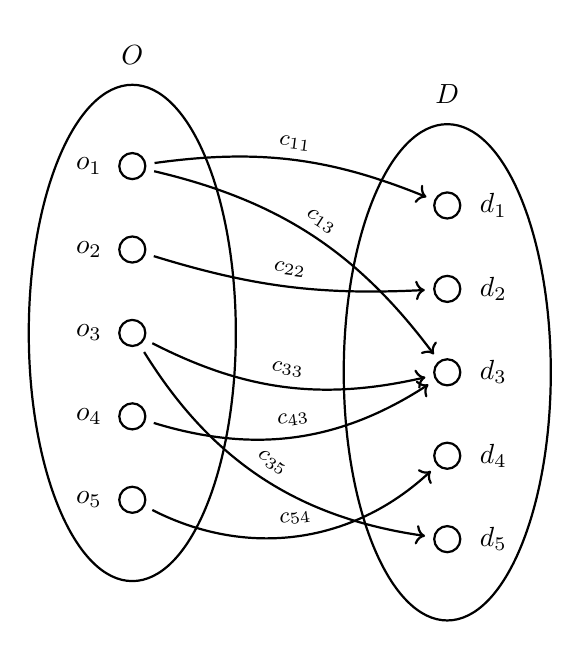
\begin{tikzpicture}[thick,
  every node/.style={draw,circle},
  ssnode/.style={},
  fsnode/.style={},
  every fit/.style={ellipse,draw,inner sep=-2pt,text width=2cm},
  ->,shorten >= 3pt,shorten <= 3pt,
  every edge quotes/.append style={font=\footnotesize,auto,sloped,draw=none,
  fill=none, text=black,inner sep=0pt,outer sep=0pt,minimum width=0pt,minimum height=0pt},
]

% the vertices of U
\begin{scope}[start chain=going below,node distance=7mm]
\foreach \i in {1,2,...,5}
\node[fsnode,on chain] (o\i) [label=left: $o_{\i}$] {};
\end{scope}

% the vertices of V
\begin{scope}[xshift=4cm,yshift=-0.5cm,start chain=going below,node distance=7mm]
\foreach \i in {1,2,...,5}
\node[ssnode,on chain] (d\i) [label=right: $d_{\i}$] {};
\end{scope}

% the set U
\node [fit=(o1) (o5),label=above:$O$] {};
% the set V
\node [fit=(d1) (d5),label=above:$D$] {};

% the edges
\draw (o1) edge["$c_{11}$", bend left = 15] (d1);
\draw (o2) edge["$c_{22}$", bend right = 10] (d2);
\draw (o3) edge["$c_{33}$", bend right = 20] (d3);
\draw (o1) edge["$c_{13}$", bend left = 20] (d3);
\draw (o4) edge["$c_{43}$", bend right = 25] (d3);
\draw (o3) edge["$c_{35}$", bend right = 25] (d5);
\draw (o5) edge["$c_{54}$", bend right = 35] (d4);
\end{tikzpicture} 
\end{center}


Il numero di variabili corrisponde al numero di archi del grafo. Quindi detti
$m$ e $n$ il numero di nodi origine e destinazione,
avremo $m\cdot n$ variabili. La funzione obiettivo sarà $$min f(x) = 
\sum_{i = 1}^n \sum_{j = 1}^m c_{ij} x_{ij}$$, dove $x_{ij}$ è la variabile che 
indica la quantità di trasporto da $i$ a $j$; mentre $c_{ij}$ indica il costo 
per percorrere il percorso $i \rightarrow j$.\\

I vincoli vengono dati dalla quantità richiesta $q_d$ di ogni nodo destinazione
$d \in D$. Ad esempio, nella prima destinazione
tutti gli archi entranti devono soddisfare la quantità richiesta $q_1$. Quindi 
la somma della merce che entra in $d_1$ deve essere uguale a $q_1$. 
\begin{equation*}
  \sum_{i = 1}^m x_{ij} \geq q_j \; \forall j \in \{1,2,3,4,5\} 
\end{equation*}

Un altro vincolo è sugli archi uscenti dalle sorgenti. Non è possibile superare
la quantità disponibile $q_o$. 
\begin{equation*}
  \sum_{j = 1}^n x_{ij} \leq q_i \; \forall i \in \{1,2,3,4,5\} 
\end{equation*}

Se le quantità nei nodi origine sono minori delle quantità nei nodi di 
destinazioni allora il problema è inammisibile.Per avere una soluzione ottima,
basta sostituire il vincolo di maggiore uguale con il vincolo di uguaglianza.

\paragraph{Esempio}
Un'azienda elettrica possiede tre centrali che devono soddisfare le esigenze di 
4 città. La tabella \ref{tab:capacita} mostra la capacità di produzione delle centrali e 
la domanda delle città.

\begin{table}[h]
  \centering  
  \begin{tabular}{|c|c|c|c|}
    \hline
    & $Cent_1$ & $Cent_2$ & $Cent_3$ \\ 
    \hline 
    Capacità & 35.000.000 & 50.000.000 & 40.000.0 \\
    \hline
  \end{tabular}
  \caption{Capacità delle centrali}
  \label{tab:capacita}
\end{table}

Il picco di domanda delle 4 città è riportato in tabella \ref{tab:domanda}.
\begin{table}[h]
  \centering  
  \begin{tabular}{|c|c|c|c|c|}
    \hline
    & $C_1$ & $C_2$ & $C_3$ & $C_4$ \\ 
    \hline 
    Domanda & 45.000.000 & 20.000.000 & 30.000.000 & 30.000.000 \\
    \hline
  \end{tabular}
  \caption{Domanda delle città}
  \label{tab:domanda}
\end{table}

Infine, nella tabella seguente è riportato il costo per trasportare 1 milione 
di kWh da una centrale ad una città.
\begin{table}[h]
  \centering  
  \begin{tabular}{|c|c|c|c|c|}
    \hline
    & $C_1$ & $C_2$ & $C_3$ & $C_4$ \\ 
    \hline 
    $Cent_1$ & 8 & 6 & 10 & 8 \\
    \hline
    $Cent_2$ & 9 & 12 & 13 & 7 \\
    \hline
    $Cent_3$ & 14 & 9 & 16 & 5 \\
    \hline
  \end{tabular}
  \caption{Costo per trasportare 1 milione di kWh da una centrale ad una città}
  \label{tab:costo}
\end{table}
Quale è il modo ottimale d rifornire le città?\\

Di seguito è riportato il grafo del problema in cui sono stati tracciati gli 
archi solo per la prima sorgente.

\begin{center}
\begin{tikzpicture}[thick,
  every node/.style={draw,circle},
  ssnode/.style={},
  fsnode/.style={},
  every fit/.style={ellipse,draw,inner sep=-2pt,text width=2cm},
  ->,shorten >= 3pt,shorten <= 3pt,
  every edge quotes/.append style={font=\footnotesize,auto,sloped,draw=none,
  fill=none, text=black,inner sep=0pt,outer sep=0pt,minimum width=0pt,minimum 
  height=0pt},
]

% the vertices of U
\begin{scope}[start chain=going below,node distance=7mm]
\foreach \i in {1,2,...,3}
\node[fsnode,on chain] (o\i) [label=left: $o_{\i}$] {};
\end{scope}

% the vertices of V
\begin{scope}[xshift=4cm,yshift=-0.5cm,start chain=going below,node distance=7mm]
\foreach \i in {1,2,...,4}
\node[ssnode,on chain] (d\i) [label=right: $d_{\i}$] {};
\end{scope}

% the set U
\node [fit=(o1) (o5),label=above:$Centrali$] {};
% the set V
\node [fit=(d1) (d5),label=above:$Citta$] {};

% the edges
\draw (o1) edge["$8$", bend left = 15] (d1);
\draw (o1) edge["$6$", bend right = 10] (d2);
\draw (o1) edge["$10$", bend right = 20] (d3);
\draw (o1) edge["$8$", bend right = 20] (d4);
\end{tikzpicture} 
\label{fig:grafo_esempio_trasporto}
\end{center}

Innanzitutto, come detto in teoria, bisogna creare le variabili di decisione 
$x_{ij}$ che rappresentano la quantità di energia che viene trasportata dalla 
centrale $i$ alla città $j$.\\
Quindi per ottenere i vincoli del problema bisogna imporre la quantità delle 
frecce entranti nei nodi destinazione uguale alla quantità richiesta dai nodi 
destinazione.  
\begin{equation*}
  \sum_{i=1}^3 x_{ij} = d_j \quad \forall j \in \{1,2,3,4\} 
\end{equation*}
Esplicitando la sommatoria si ottengono le seguenti equazioni:
\begin{equation*}
  \begin{cases}
  x_{11} + x_{21} + x_{31} = 45.000.000\\
  x_{12} + x_{22} + x_{32} = 20.000.000\\
  x_{13} + x_{23} + x_{33} = 30.000.000\\
  x_{14} + x_{24} + x_{34} = 30.000.000\\
  \end{cases}
\end{equation*}

Inoltre, per ogni nodo sorgente, la quantità di energia che viene trasportata 
deve essere uguale o inferiore a quella prodotta dalla centrale. Si ottengono 
così le seguenti disequazioni:
\begin{equation*}
  \sum_{j=1}^4 x_{ij} \leq c_i \quad \forall i \in \{1,2,3\} 
\end{equation*}
Esplicitnado la sommatoria si ottengono le seguenti disequazioni:

\begin{equation*}
  \begin{cases}
  x_{11} + x_{12} + x_{13} + x_{14} \leq 50.000.000\\
  x_{21} + x_{22} + x_{23} + x_{24} \leq 30.000.000\\
  x_{31} + x_{32} + x_{33} + x_{34} \leq 40.000.000\\
  \end{cases}
\end{equation*}

Mentre la funzione obiettivo è data dalla somma dei costi di trasporto che si 
vuole minimizzare ed è data dalla somma dei prodotti tra le variabili di 
decisione e i costi di trasporto:
\begin{equation*}
  \min \sum_{i=1}^3 \sum_{j=1}^4 x_{ij} c_{ij}
\end{equation*}
Ad esempio, per il primo nodo sorgente la funzione obiettivo è:
\begin{equation*}
  \min
  \begin{pmatrix}
    8x_{11} + 6x_{12} + 10x_{13} + 8x_{14} +\\ 
    9x_{21} + 12x_{22} + 13x_{23} + 7x_{24} +\\
    14x_{31} + 9x_{32} + 16x_{33} + 5x_{34} \\
  \end{pmatrix}
\end{equation*}


\paragraph{Esempio: problema del trasporto con più livelli}
Un’industria produce un preparato chimico utilizzando due impianti di produzione
$I_1$, $I_2$. Da questi impianti, il preparato chimico prodotto viene 
trasportato in due magazzini $M_1$, $M_2$ che si trovano in differenti località. 
In questi magazzini una parte del preparato è venduta all’ingrosso direttamente, 
un’altra parte viene inviata a quattro centri di distribuzione $D_1, D_2, D_3, 
D_4$ che effettuano la vendita al dettaglio. Questi centri necessitano 
rispettivamente di almeno 150, 190, 220, 170 quintali di preparato chimico che 
vendono rispettivamente a 350, 280, 200, 270 euro al quintale. La tabella 
\ref {tab:costi_trasporto_magazzini} riporta i costi necessari per trasportare
un quintale di preparato da ciascun impianto a ciascun magazzino.

\begin{table}
  \centering
  \begin{tabular}{|c|c|c|}
    \hline
    & $M_1$ & $M_2$ \\ 
    \hline 
    $I_1$ & 21 & 25 \\
    $I_2$ & 27 & 22 \\
    \hline
  \end{tabular}
  \caption{Costi di trasporto nei magazzini}
  \label{tab:costi_trasporto_magazzini}
\end{table}

L’impianto di produzione $I_1$ può fabbricare al più 3000 quintali di preparato,
l’impianto $I_2$ può fabbricare al più 2000 quintali di preparato.
I prezzi di vendita all’ingrosso effettuati presso i magazzini $M_1$ e $M_2$ sono
rispettivamente di euro 150 e 170 al quintale. Per ragioni commerciali i 
quantitativi di preparato chimico venduti all’ingrosso in ciascun magazzino
devono essere pari ad almeno 500 quintali ed inoltre tutto il preparato
contenuto nei magazzini dovrà essere o venduto o trasportato ai centri di 
distribuzione per non avere rimanenze non vendute. Costruire un modello lineare
che permetta di determinare le quantità di preparato chimico che devono essere
prodotte in ciascun impianto e come esse devono essere ripartite tra i magazzini
e i centri di distribuzione in modo da massimizzare il profitto netto complessivo.

Nella tabella \ref{tab:costi_trasporto_centri} si riportano i costi necessari
per trasportare un quintale di preparato chimico da ciascun magazzino a ciascun 
di distribuzione.\\

\begin{table}
  \centering
  \begin{tabular}{|c|c|c|c|c|}
    \hline
    & $D_1$ & $D_2$ & $D_3$ & $D_4$\\ 
    \hline 
    $M_1$ & 33 & 31 & 36 & 30 \\
    $M_2$ & 27 & 30 & 28 & 31 \\
    \hline
  \end{tabular}
  \caption{Costi di trasporto nei centri di distribuzione}
  \label{tab:costi_trasporto_centri}
\end{table}

Questo problema può essere modellato come un problema di trasporto con più 
livelli e pertanto necessita di due insiemi di variabili decisionali: uno per 
il trasporto dai due impianti di produzione ai due magazzini e uno per il 
trasporto dai due magazzini ai quattro centri di distribuzione. Le variabili 
sono $x_{ij}$ dove $i$ indica l'impianto e $j$ il magazzino; mentre con $y_{lk}$
si indica la quantità di materiale trasportato dai magazzini $l$ ai centri di 
distribuzione $k$. Inoltre, bisogna considerare anche la possibilità di vendere 
il preparato all'ingrosso nei magazzini. Per fare ciò è utile considerare i 
magazzini come dei centri di distribuzione il cui costo di trasporto è $0$ e 
si introducono due variabili $z_1$ e $z_2$ per indicare le quantità vendute 
all'ingrosso.

Infine, il problema può essere modellato con il grafo mostrato in figura 
\ref{fig:grafo_3_lv}.

\begin{figure}
  \centering
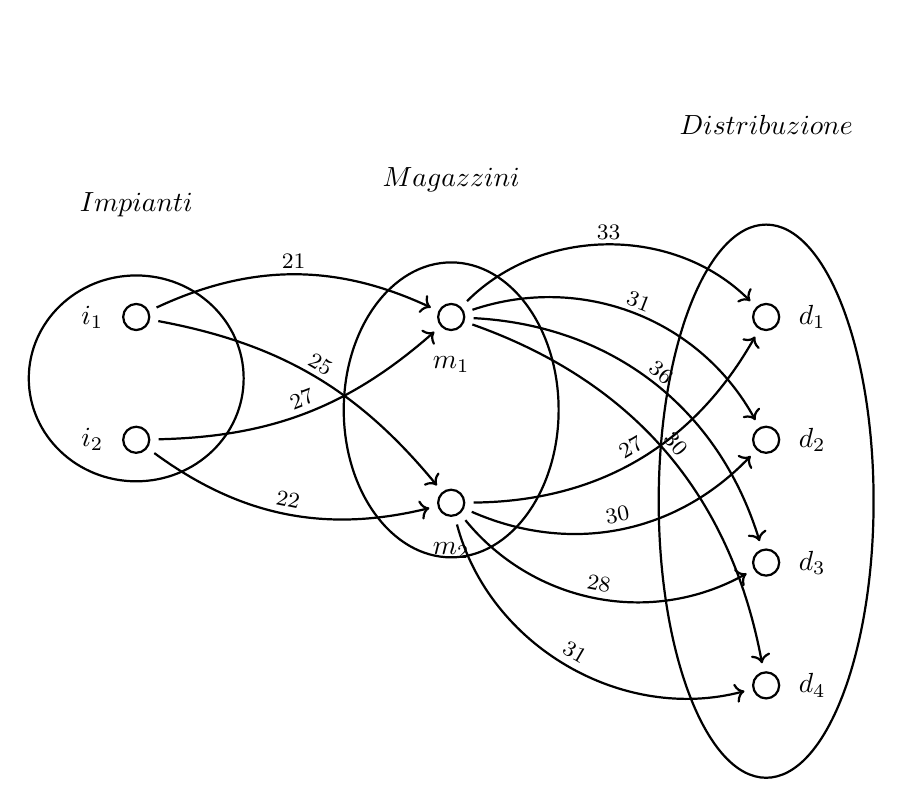
\begin{tikzpicture}[thick,
  every node/.style={draw,circle},
  ssnode/.style={},
  fsnode/.style={},
  amnode/.style={},
  every fit/.style={ellipse,draw,inner sep=-1pt,text width=2cm},
  ->,shorten >= 3pt,shorten <= 3pt,
  every edge quotes/.append style={font=\footnotesize,auto,sloped,draw=none,
  fill=none, text=black,inner sep=0pt,outer sep=0pt,minimum width=0pt,minimum 
    height=0pt},
]

% the vertices of U
\begin{scope}[start chain=going below,node distance=12mm]
\foreach \i in {1,2}
\node[fsnode,on chain] (i\i) [label=left: $i_{\i}$] {};
\end{scope}

% the vertices of V
\begin{scope}[xshift=4cm,start chain=going below,node distance=20mm]
\foreach \i in {1,2}
\node[ssnode,on chain] (m\i) [label=below: $m_{\i}$] {};
\end{scope}

% the vertices of V
\begin{scope}[xshift=8cm,start chain=going below,node distance=12mm]
\foreach \i in {1,2,...,4}
\node[amnode,on chain] (d\i) [label=right: $d_{\i}$] {};
\end{scope}

% the set U
\node [fit=(i1) (i2),label=above:$Impianti$] {};
% the set V
\node [fit=(m1) (m2),label=above:$Magazzini$] {};
\node [fit=(d1) (d4),label=above:$Distribuzione$] {};

% livello 1
\draw (i1) edge["$21$", bend left = 25] (m1);
\draw (i1) edge["$25$", bend left = 20] (m2);
\draw (i2) edge["$27$", bend right = 20] (m1);
\draw (i2) edge["$22$", bend right = 25] (m2);

% livello 2
\draw (m1) edge["$33$", bend left = 45] (d1);
\draw (m1) edge["$31$", bend left = 40] (d2);
\draw (m1) edge["$36$", bend left = 35] (d3);
\draw (m1) edge["$30$", bend left = 30] (d4);

\draw (m2) edge["$27$", bend right = 30] (d1);
\draw (m2) edge["$30$", bend right = 35] (d2);
\draw (m2) edge["$28$", bend right = 40] (d3);
\draw (m2) edge["$31$", bend right = 45] (d4);
\end{tikzpicture} 
\label{fig:grafo_3_lv}
\caption{Rappresentazione grafica del problema}
\end{figure}

Partendo dalla fine, troviamo che le richieste dei singoli centri di 
distribuzione $d_i$ devono essere rispettati. Questo genera il seguente sistema 
di equazioni:

\begin{equation*}
  \begin{cases}
  y_{11} + y_{21} \leq 150\\
  y_{12} + y_{22} \leq 190\\
  y_{13} + y_{23} \leq 220\\
  y_{14} + y_{24} \leq 170\\
  \end{cases}
\end{equation*}
Invece, considerando gli impianti iniziali si ha che le consegne ai magazzini 
non devono superare le quantità prodotte:

\begin{equation*}
  \begin{cases}
  x_{11} + x_{12} \leq 3000\\
  x_{21} + x_{22} \leq 2000\\
  \end{cases}
\end{equation*}

Inoltre, bisogna imporre che le quantità vendute all'ingrosso nei singoli 
magazzini sia almeno 500:

\begin{equation*}
  \begin{cases}
  z_1 \geq 500 \\
  z_2 \geq 500\\
  \end{cases}
\end{equation*}

La funzione obiettivo sarà quindi data dalla differenza tra ricavi e costi. 
In particolare, i ricavi delle vendite presso i centri distribuzione sono:

\begin{equation*}
  \begin{pmatrix}
    350(y_{11} + y_{21}) + \\
    280(y_{12} + y_{22}) + \\
    200(y_{13} + y_{32}) + \\
    270(y_{14} + y_{42})  \\
  \end{pmatrix}
\end{equation*}

Mentre quelli dati dalla vendita all'ingrosso sono:
\begin{equation*}
    150z_1 + 170z_2
\end{equation*}

Infine, bisogna imporre che la merce ricevuta dai magazzini sia uguale a quella 
in uscita.

\begin{equation*}
  \begin{cases}
    x_{11} + x_{21} = z_1 + y_{11} + y_{12} + y_{13} + y_{14} \\
    x_{21} + x_{22} = z_2 + y_{21} + y_{22} + y_{23} + y_{24} \\
  \end{cases}
\end{equation*}



I costi invece sono dati dal trasporto delle quantità in $M_1$ e $M_2$.
\begin{equation*}
  21x_{11} + 25x_{12} + 27x_{21} + 22x_{22} 
\end{equation*}

mentre quelli per trasportare il preparato da $M_1$ e $M_2$ a $D_1,D_2,D_3,D_4$
sono:
\begin{equation*}
  \begin{pmatrix}
  33y_{11} + 31y_{12} + 36x_{13} + 30x_{14} + \\
  27y_{21} + 30y_{22} + 28x_{23} + 31x_{24}  \\
  \end{pmatrix}
\end{equation*}

Quindi in definitiva la funzione obiettivo sarà:
\begin{equation*}
  \max
  \begin{pmatrix}
  350(y_{11} + y_{21}) + 280(y_{12} + y_{22}) + 200(y_{13} + y_{32}) + \\ 
  270(y_{14} + y_{42}) + 150z_1 + 170z_2 - 21x_{11} - 25x_{12} -\\ 
  27x_{21} - 22x_{22} - 33y_{11} - 31y_{12} - 36x_{13} - \\ 
  30x_{14} - 27y_{21} - 30y_{22} - 28x_{23} - 31x_{24}
\end{pmatrix}
\end{equation*}

\subsection{Problemi non lineari riconduibili a problemi lineari}
\subsubsection{Problemi con funzione obiettivo di tipo $\min (\max e(x)$)}
Si consideri un problema di programmazione matematica in cui i vincoli sono 
lineari, ma la funzione obiettivo sia del tipo: $$\max \min {e_1(x), e_2(x),
\dots,e_q(x)}$$. Per risolvere il problema, si riconduce il problema spostando 
la funzione interna ($\min$ per il caso max-min e max per il caso $min-max$) 
all'interno di un vincolo che genera un insieme di disequazioni del tipo 
$y \leq e_i \forall i = 1..q$. La funzione obiettivo diventa $\max y$, dove 
$y = \min{e_1(x),e_2(x),\dots,e_q(x)}$.

\paragraph{Esempio}
Un mangime è ottenuto miscelando tre componenti che possono essere lavorate
su quattro linee di produzione differenti. La miscela è fatta esattamente da un
terzo della prima componente, un terzo della seconda e un terzo della terza
componente. Ogni linea e dotata di una limitata capacita di ore di lavorazione e
una diversa produttività (unità di componente per ogni ora), come indicato nella 
seguente tabella. Si vuole determinare il numero di ore di lavorazione di 
ciascuna componente su ciascuna linea di produzione in modo da massimizzare la
quantità di mangime.

Sia $x_{ij}$ la quantità di componente $j$ prodotta sulla linea $i$.
I vincoli sono dati delle linee di produzione e sono:
\begin{align*}
  10x_{11} + 15x_{12} + 5x_{13} &\leq 100\\ 
  15x_{21} + 10x_{22} + 5x_{23} &\leq 150\\ 
  20x_{31} + 5x_{32} + 10x_{33} &\leq 80\\ 
  10x_{41} + 15x_{42} + 20x_{43} &\leq 200\\ 
  x_{ij} &\geq 0 \quad \forall i,j \in \{1,2,3,4\}
\end{align*}

La funzione obiettivo è:

\subsubsection{Problemi con funzione obiettivo del tipo $ |e(x)|$}
Si consideri un problema di programmazione matematica con vincoli lineari in 
cui la funzione obiettivo è del tipo: $$\min |e(x)|$$. Per risolvere il 
problema, si introduce una variabile $y = \max{e(x), -e(x)}$ e la funzione 
obiettivo diventa $\min y$. Inoltre, si aggiungono i vincoli $y \geq e(x)$ e 
$y \geq -e(x)$

\section{Soluzione dei problemi di programmazione lineare}
In questa sezione, vengono analizzati i metodi per risolvere i problemi di 
programmazione lineare. \\ In particolare, per i problemi a 2 variabili
è possibile trovare una soluzione grafica, mentre per quelli a
più variabili è necessario utilizzare altre strategie che generalizzano
il caso bidimensionale.\\ 
Innanzitutto, sono fornite le definizioni di insieme convesso e di vertice 
sulle quali si basa il teorema fondamentale della programmazione lineare.

\paragraph{Combinazione convessa}
  -Dati $x,y\in \Re^n$ e $\lambda \in [0,1]$, si dice combinazione convessa 
  di $x,y$ un qualsiasi punto ottenuto:$$\lambda x + (1-\lambda)y$$
  

\paragraph {Insieme convesso}
-  Un insieme $\Theta$ è detto convesso se comunque presi due punti
  appartenentiall'insieme, il segmento che li congiunge appartiene interamente
  all’insieme.Utilizzando questa definizione è possibile dimostrare che
  l’intersezione di un numero finito di insiemi convessi è un insieme
  convesso.


In ogni caso, i due metodi si basano sull'utilizzo del teorema seguente:

\paragraph{Teorema fondamentale della programmazione lineare}
  IIn un problema di programmazione lineare si possono presentare i seguenti 
  casi:
  \begin{itemize}
    \item la regione ammissibile è vuota $\rightarrow$ il problema è non ha 
      soluzione;
    \item la regione ammissibile è illimitata e la funzione obiettivo è
      illimitata nello stesso verso $\rightarrow$ il problema non ha soluzione;
    \item se non ci si trova in nessuno dei casi precedenti, allora il problema 
      ha una soluzione ottima che può essere unica o non unica (infinite 
      soluzioni). Il dominio di ammissibilità risulta essere 
      una regione convessa del piano cartesiano e almeno una delle soluzioni si 
      trova in un vertice del poligono convesso costituito dalla regione
      ammissibile;
  \end{itemize}
  Il teorema della programmazione lineare afferma che una e una sola delle 
  seguenti affermazioni è vera.

\subsection{Soluzione grafica dei problemi di ottimizzazione}
Quando si ha un problema lineare in due dimensioni questo può essere risolto 
facilmente per via grafica sapendo che un'equazione individua una retta; mentre
una disequazione individua un semipiano.\\ 
Infatti, un problema di programmazione lineare con i suoi vincoli individua 
una regione dello spazio cartesiano delimitando il dominio di ammissibilità 
delle soluzioni; mentre con la funzione obiettivo determina quale delle 
soluzioni disponibili (se esistono) verifica il vincolo di $\max$ o $\min$.\\ 

\paragraph{Esempio: problema soluzione ottima unica}
Sia dato il seguente problema di programmazione lineare:
\begin{align*}
  obj: \max z &= 5x_1+10x_2\\
  v1: &\quad 10x_1 + 5x_2  \leq 25 \\
  v2: &\quad 4x_1 + 10x_2  \leq 20 \\
  v3: &\quad x_1 + 1.5x_2  \leq 4.5\\
  x_1,x_2 \geq 0
\end{align*}

Innanzitutto, si rappresenta il dominio di ammissibilità dato dai vincoli 
del problema, come mostrato in \ref{fig:opt_ammissibilità}.

\begin{figure}
  \center
  \label{fig:opt_ammissibilità}
  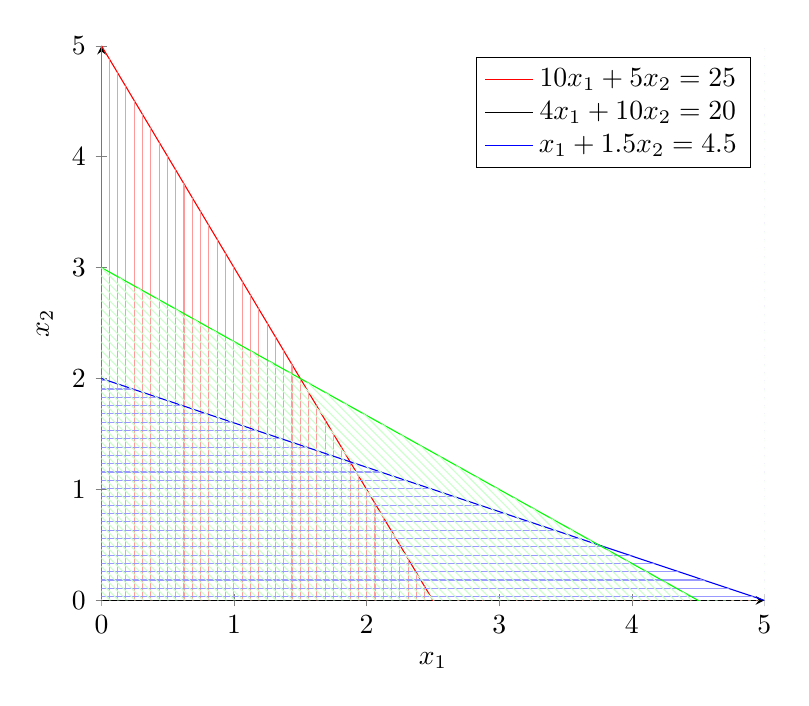
\begin{tikzpicture}
    \begin{axis}[
      axis lines = left,
      xlabel = \(x_1\),
      ylabel = \(x_2\),
      ymin=0,
    ]
      %v1
      \addplot [
        domain=0:10, 
        samples=10, 
        color=red,
        name path=v1,
      ]
      {5-2*x};
      \addplot [
        draw=none,pattern= vertical lines, pattern color = red!40, domain=0:10
      ]
      {5-2*x} \drawle;

      %v2
      \addplot [
        domain=0:10, 
        samples=10, 
        color=blue,
        name path=v2,
      ]
        {2 - (4/10)*x };
      
      \addplot [
        draw=none,pattern= horizontal lines, pattern color = blue!40, domain=0:10
      ]{2 - (4/10)*x } \drawle;
      
      %v3
      \addplot [
        domain=0:10, 
        samples=10, 
        color=green,
        name path=v3,
        ]
        {3 - (1/1.5)*x };
      
      \addplot [
        draw=none,pattern=north west lines, pattern color = green!20, domain=0:10
      ]{3 - (1/1.5)*x } \drawle;
      
      \addlegendentry{\(10x_1 + 5x_2 = 25\)}
      \addlegendentry{\(4x_1 + 10x_2 = 20\)}
      \addlegendentry{\(x_1 + 1.5x_2 = 4.5\)}

    \end{axis}
  \end{tikzpicture}
  \caption{Individuazione del dominio di ammissibilità}
\end{figure}

Successivamente, si tracciano le linee di livello della funzione obiettivo che,
essendo nel caso lineare, saranno del tipo $\max {ax_1+bx_2 = k}$ e quindi 
parallele tra loro. Come affermato nel teorema fondamentale, la soluzione ottima 
laddove esistesse, si trova sulla frontiera del poliedro. In figura
\ref{fig:opt_linee_di_livello}, sono mostrate 2 linee di livello: partendo da 
destra, $k=30$ e si nota che non ricade nel dominio di ammissibilità; mentre 
quella successiva ($k=21.875$) interseca il poliedro delimitato nel vertice 
in alto a destra. Quindi il valore di $k$ che ha generato la linea rappresenta 
l'ottimo del problema a cui si arriva assegnando alle variabili $x_1$ e $x_2$ 
i valori di $(1.875,1.25)$.
\begin{figure}
  \center
  \label{fig:opt_linee_di_livello}
  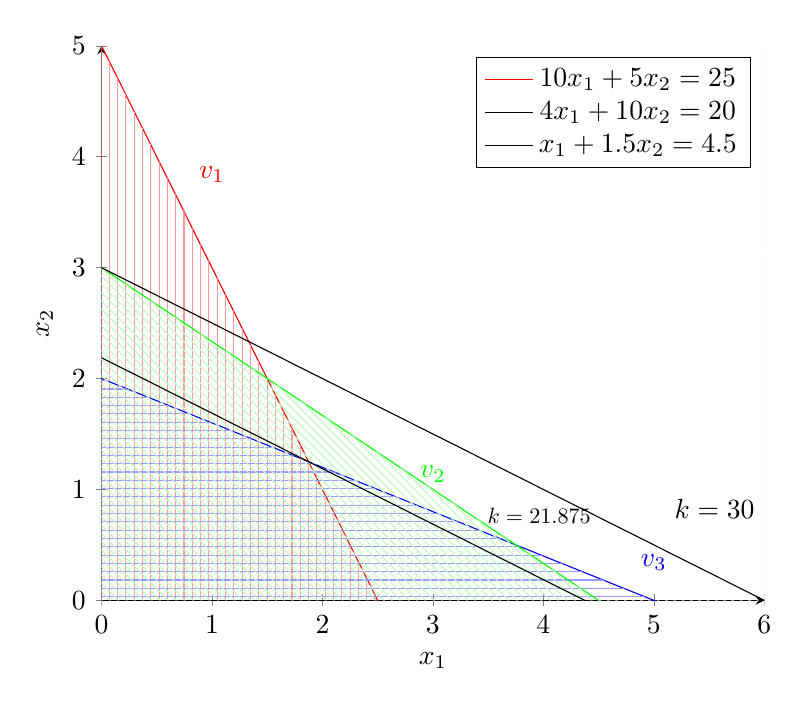
\begin{tikzpicture}
    \begin{axis}[
      axis lines = left,
      xlabel = \(x_1\),
      ylabel = \(x_2\),
      ymin=0,
      xmax=6,
    ]
      %v1
      \addplot [
        domain=0:10, 
        samples=10, 
        color=red,
      ]
      {5-2*x}; 
      \addlegendentry{\(10x_1 + 5x_2 = 25\)}

      \addplot [
        draw=none,
        pattern= vertical lines, 
        pattern color = red!40, 
        domain=0:10
      ]
      {5-2*x} \drawle;
      \addplot[no marks] 
        coordinates{(1,4)} node[pos=0.25,below,color=red] {$v_1$};

      %v2
      \addplot [
        domain=0:10, 
        samples=10, 
        color=blue,
        name path=v2,
      ]
        {2 - (4/10)*x };
      
      \addlegendentry{\(4x_1 + 10x_2 = 20\)}
      \addplot [
        draw=none,pattern= horizontal lines, pattern color = blue!40, domain=0:10
      ]{2 - (4/10)*x } \drawle;
      \addplot[no marks] 
        coordinates{(3,1.3)} node[below,color=green] {$v_2$};
      %v3
      \addplot [
        domain=0:10, 
        samples=10, 
        color=green,
        name path=v3,
        ]
        {3 - (1/1.5)*x };
      
      \addlegendentry{\(x_1 + 1.5x_2 = 4.5\)}
      \addplot [
        draw=none,pattern=north west lines, pattern color = green!25, domain=0:10
      ]{3 - (1/1.5)*x } \drawle;

      \addplot[no marks] 
        coordinates{(5,0.5)} node[pos=0.25,below,color=blue] {$v_3$};

      \addplot [
        domain=0:10, 
        samples=10, 
        color=black,
      ]
      {3-1/2*x};

      \addplot[no marks] 
        coordinates{(6,1)} node[below left] {$k=30$};

      \addplot [
        domain=0:10, 
        samples=10, 
        color=black,
      ]
      {2.1875-1/2*x};
      \addplot[no marks] 
        coordinates{(4.5,0.9)} node[scale=0.8,below left] {$k=21.875$};
    \end{axis}
  \end{tikzpicture}
  \caption{Tracciamento delle linee di livello (in nero): 
  partendo da destra $k=30$, la successiva ha $k=21.875$}
\end{figure}

\paragraph{Esempio: regione di ammissibilità vuota}
Sia dato il seguente problema di programmazione lineare:

\begin{align*}
  obj: \max z &= 4x_1+10x_2\\
  v1: &\quad 10x_1 + 5x_2  \leq 25 \\
  v2: &\quad 4x_1 + 10x_2  \leq 20 \\
  v3: &\quad x_1 + 1.5x_2  \geq 4.5\\
  x_1,x_2 \geq 0
\end{align*}

La figura \ref{fig:prob_inammissibile} mostra che non esiste in una regione del 
piano in cui tutti i vincoli sono soddisfatti. Pertanto, il problema non ha 
soluzione ammissibile.

\begin{figure}
  \center
  \label{fig:prob_inammissibile}
  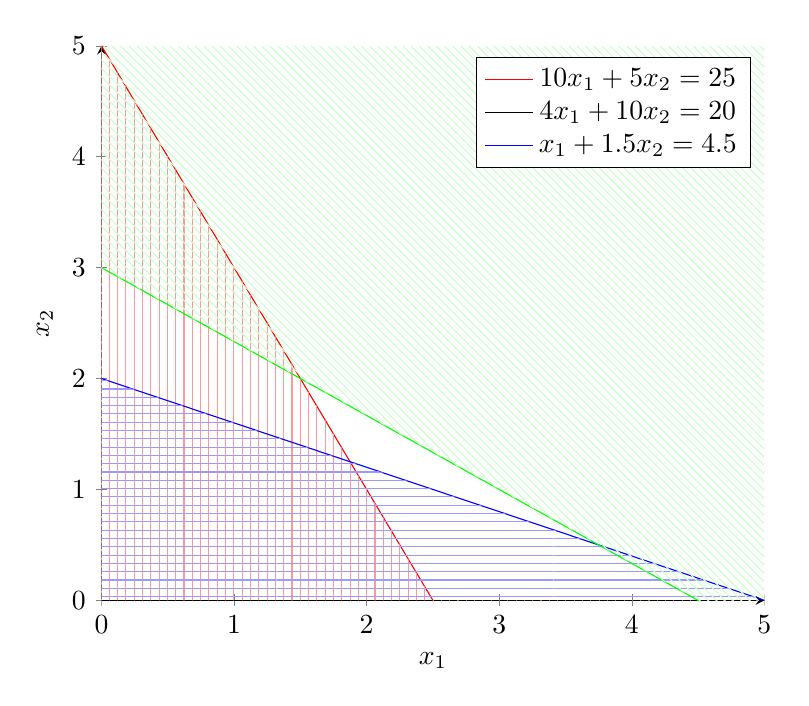
\begin{tikzpicture}
    \begin{axis}[
      axis lines = left,
      xlabel = \(x_1\),
      ylabel = \(x_2\),
      ymin=0,
    ]
      %v1
      \addplot [
        domain=0:10, 
        samples=10, 
        color=red,
        name path=v1,
      ]
      {5-2*x};
      \addplot [
        draw=none,pattern= vertical lines, pattern color = red!40, domain=0:10
      ]
      {5-2*x} \drawle;

      %v2
      \addplot [
        domain=0:10, 
        samples=10, 
        color=blue,
        name path=v2,
      ]
        {2 - (4/10)*x };
      
      \addplot [
        draw=none,pattern= horizontal lines, pattern color = blue!40, domain=0:10
      ]{2 - (4/10)*x } \drawle;
      
      %v3
      \addplot [
        domain=0:10, 
        samples=10, 
        color=green,
        name path=v3,
        ]
        {3 - (1/1.5)*x };
      
      \addplot [
        draw=none,pattern=north west lines, pattern color = green!20, domain=0:10
      ]{3 - (1/1.5)*x } \drawge;
      
      \addlegendentry{\(10x_1 + 5x_2 = 25\)}
      \addlegendentry{\(4x_1 + 10x_2 = 20\)}
      \addlegendentry{\(x_1 + 1.5x_2 = 4.5\)}

    \end{axis}
  \end{tikzpicture}
  \caption{Dominio di ammissibilità di ammissibilità inesistente}
\end{figure}

\paragraph{Esempio: dominio di ammissibilità illimitato con soluzione ottima
  finita}
Sia dato il seguente problema di programmazione lineare:

\begin{align*}
  obj: \max z &= 5x_1+10x_2\\
  v1: &\quad 10x_1 + 5x_2  \leq 25 \\
  v2: &\quad 4x_1 + 10x_2  \leq 20 \\
  v3: &\quad x_1 + 1.5x_2  \leq 25\\
  x_2 \geq 0
\end{align*}

Si noti come solo la variabile $x_2$ sia positiva, mentre la $x_1$ può
spaziare su tutto l'asse reale. Come mostrato in figura \ref{fig:dom_illimitato}
il dominio si estende verso $\-inf$ illimitamente, ma la soluzione resta come 
nel caso di precedente nel vertice in alto a destra.

\begin{figure}
  \center
  \label{fig:dom_illimitato}
  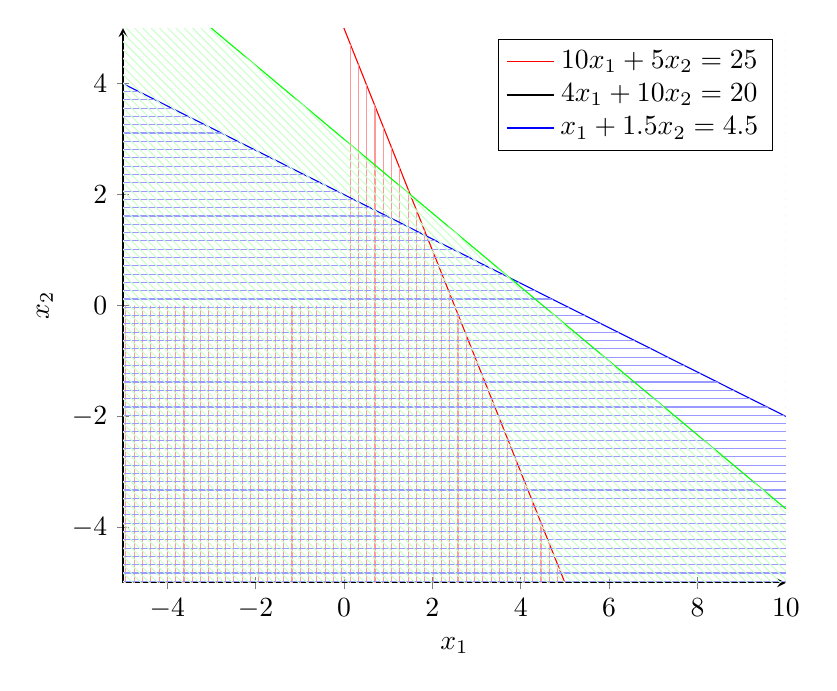
\begin{tikzpicture}
    \begin{axis}[
      axis lines = left,
      xlabel = \(x_1\),
      ylabel = \(x_2\),
      ymin=-5,
      ymax=5,
      xmin=-5
    ]
      %v1
      \addplot [
        domain=-5:10, 
        samples=10, 
        color=red,
        name path=v1,
      ]
      {5-2*x};
      \addplot [
        draw=none,pattern= vertical lines, pattern color = red!40, domain=0:10
      ]
      {5-2*x} \drawle;

      %v2
      \addplot [
        domain=-5:10, 
        samples=10, 
        color=blue,
        name path=v2,
      ]
        {2 - (4/10)*x };
      
      \addplot [
        draw=none,pattern= horizontal lines, pattern color = blue!40, 
        domain=-5:10
      ]{2 - (4/10)*x } \drawle;
      
      %v3
      \addplot [
        domain=-5:10, 
        samples=10, 
        color=green,
        name path=v3,
        ]
        {3 - (1/1.5)*x };
      
      \addplot [
        draw=none,pattern=north west lines, pattern color = green!20,
        domain=-5:10
      ]{3 - (1/1.5)*x } \drawle;
      
      \addlegendentry{\(10x_1 + 5x_2 = 25\)}
      \addlegendentry{\(4x_1 + 10x_2 = 20\)}
      \addlegendentry{\(x_1 + 1.5x_2 = 4.5\)}

    \end{axis}
  \end{tikzpicture}
  \caption{Dominio di ammissibilità illimitato}

\end{figure}
\subsection{Problemi con $n$ variabili: algoritmo del simplesso}
L'algoritmo del simplesso comincia con enumerare tutti i vertici del poliedro poi 
utilizza il concetto di derivata direzionale per capire se esiste un vertice migliore. \\ 
L'algoritmo del simplesso funziona solo con variabili positive. Nel caso in cui 
si avessero variabili non ristrette nel segno, si può effettuare una trasformazione 
della funzione obiettivo con una sostituzione di variabili con una sostituzione del tipo 
$x_i = x_i^+ - x_i^-$ dove $x_i^+$ e $x_i^-$ sono due nuove variabili positive.
Questo problema si ripresenta anche quando i termini noti sono negativi. Per ogni 
termine noto bisogna moltiplicare per $-1$ primo e secondo membro prima di partire 
con l'applicazione dell'algoritmo del simplesso.\\

Si dimostra che i vertici di un dominio di ammissibilità di un problema PL 
corrispondono a particolari soluzioni e si ottengono da sistemi di equazioni lineari 
ottenuto dalle disequazioni del problema PL
\begin{align*}
  \min z &= c_1x_1 + c_2x_2 + \cdots + c_n x_n\\
  s.c. &\quad a_{11}x_1 + a_{12}x_2 + \cdots + a_{1n}x_n \leq b_1\\
  &\quad a_{21}x_1 + a_{22}x_2 + \cdots + a_{2n}x_n \leq b_2\\
  &\quad \vdots\\
  &\quad a_{m1}x_1 + a_{m2}x_2 + \cdots + a_{mn}x_n \leq b_m\\
  &\quad x_1,x_2,\dots,x_n \geq 0
\end{align*}

\paragraph{Esercizio}
Una azienda deve produrre 2 profilati metallici (A e B) che richiedono l'impiego 
di manodopera, disponibile al massimo in 36 squadre. Per 
la produzione giornaliera di un lotto di A e di un lotto di B si impiegano rispettivamente 3 e 6 squadre. 
È necessario produrre tra A e B almeno 4 lotti al giorno.
Si possono impiegare due diverse tecnologie (1 e 2).
La tecnologia 1 produce al massimo 2 lotti di B per ogni lotto di A 
(cioè le produzioni di B ed A sono al massimo nel rapporto 2:1).
La tecnologia 2 produce al massimo 2 lotti di A  per ogni lotto di B (cioè le produzioni di A e B sono al massimo nel rapporto 2:1). 
Il profitto unitario è lo stesso per entrambi  i prodotti.
Si vuole determinare il piano di produzione giornaliero che massimizza il profitto totale.

Analisi: il testo di dell'esercizio non dice come calcolare il profitto, ma a noi 
interesa solo capire le soluzioni. Possiamo comunque disegnare l'insieme di ammissibilità
e le linee di livello per capire come si comporta la funzione obiettivo. Questo vale anche 
se avessi informazioni del tipo "il proffito di A è il doppio di B". Questo perchè 
posso scrivere la funzione obiettivo come $f(x) = 2Kx_1 + Kx_2$ e non mi cambia nulla.

Questo problema ha come funzione obiettivo $\max z =Kx_1 + Kx_2$ con $K$ il profitto unitario.
e come vincoli:
\begin{align*}
  3x_a + 6x_b &\leq 36\\ 
  x_b &\leq 2x_a \\
  x_a + x_b &\geq 4 \\ 
  x_a &\leq 2x_b \\
\end{align*}

Per risolvere graficamente, disegniamo l'insieme di ammissibilità e le linee di livello.
Quindi notiamo che $x_1,x_2 \geq 0$. Ogni disequazione individua un semipiano. 
Individuato il vertice ottimo, per avere le sue coordinate si può risolvere il sistema lineare 
che si ottiene intersecando le rette che rappresentano le disequazioni con cui si è
ricavato il dominio di ammissibilità.

In particolare, un sistema di disequazioni in un sistema di equazioni lineari 
tramite l'aggiunta di variabili slack. Per un vincolo $a_{ij}x_j \leq b_i$ 
si aggiunge una variabile artificiale $y_{i}$ e si sostituisce il vincolo con 
$a_{ij}x_j + y_{i} = b_i$ con $y_i \leq 0$. Per un vincolo di tipo $a_{ij}x_j \geq b_i$ 
si aggiunge una variabile artificiale $y_{i}$ e si sostituisce il vincolo con 
$a_{ij}x_j - y_{i} = b_i$ con $y_i \geq 0$.Si ottiene così un sistema di equazioni lineari 
con $m$ equazioni e $n+m$ variabili. 

% soluzioni basiche
Dato un sistema di $m$ equazioni in $n$ variabilie, si dice che una soluzione 
è \emph{basica} se presenta $n-m$ variabili nulle e $m$ variabili positive.  

Quindi l'algoritmo del simplesso salta da una soluzione basica ammissibile a un 
altra. Appena viene soddisfatto il test di ottimalità, l'algoritmo termina.

\paragraph{Esercizio} 
Sia data la seguente funzione obiettivo con vincoli:
\begin{align*}
  \max z &= 4x_1 + x_2 \\ 
  s.c. &\quad 2x_1 + x_2 \leq 2\\ 
  &\quad x_1 + 2x_2 \leq 2\\ 
\end{align*}
Conosciamo già che la soluzione si trova in uno dei vertici del dominio di ammissibilità.
Quindi, possiamo tracciare le curve parametriche che rappresentano le rette che 
definiscono il dominio di ammissibilità che saranno del tipo $4x_1 + x_2 = K$ e 
con $K=2$ troviamo il vertice sull'asse delle ascisse.\\ 

Proviamo a risolvere il problema in forma matriciale con le variabili slack.
\begin{align*}
  &\quad 4x_1 + x_2 - z = 0\\ 
  &\quad 2x_1 + x_2 + y_1 = 2\\ 
  &\quad x_1 + 2x_2 + y_2 = 2\\ 
\end{align*}

Quindi estraggo la matrice dei coefficienti del sistema. 
\begin{equation*}
  \begin{pmatrix}
    x_1 & x_2 & y_1 & y_2 & -z & b\\
    2 & 1 & 1 & 0 & 0 & 2\\ 
    1 & 2 & 0 & 1 & 0 & 2\\ 
    4 & 1 & 0 & 0 & 1 & 0\\ 
  \end{pmatrix}
\end{equation*}

Le soluzioni del sistema sono infinite. Una soluzione semplice consiste nel 
mettere $x_1=0$ e $x_2=0$, ottenendo $y_1=2$ e $y_2=2$ e $z=0$. Posso arrivare 
all'ottimo seguendo le derivate direzionali e scegliendo la direzione in cui 
la funzione obiettivo aumenta di più. Quando la funzione obiettivo non aumenta o 
la derivata direzionale è nulla si ha un vertice ottimo.\\

Posso ottenere un sistema equivalente sostituendeo con le seguenti sostituzioni: 
$R1 = R1 - \frac{1}{2}R2$ e $R2 = R2 - \frac{1}{4}R3$.\\
\begin{align*}
  \quad x_1 + \frac{1}{2}x_2 - \frac{1}{2}y_1 &= 1\\ 
  \quad \frac{3}{2}x_2 - \frac{1}{2}y_1 + y_2 &= 1\\ 
  \quad -x_2 - 2y_1 -z &= -4\\ 
\end{align*}

Ottengo così la seguente matrice dei coefficienti:
\begin{equation*}
  \begin{pmatrix}
    x_1 & x_2 & y_1 & y_2 & -z & b\\
    1 & \frac{1}{2} & \frac{1}{2} & 0 & 0 & 1\\ 
    0 & \frac{3}{2} & -\frac{1}{2} & 1 & 0 & 1\\ 
    0 & -1 & -2 & 0 & 1 & -4\\ 
  \end{pmatrix}
\end{equation*}

Posso calcolare velocemente la soluzione consideriamo le colonne che formano una 
matrice identica ($C=i\; con\; i \in {1,4,5}$) per avere $x_1=1$ e $y_2=1$ e $z=4$.\\

Con il sistema equivalente trovato, la funzione obiettivo diventa $z=-x_2-2y_1+4$.
Da qui si osserva che le derivate direzioni sono $-1$ e $-2$.

\paragraph{Esercizio}
Sia data la seguente funzione obiettivo con vincoli:
\begin{align*}
  \max z &= 11x_1 + 10x_2 \\ 
  s.c. &\quad -5x_1 + 4x_2 \leq 20\\ 
  &\quad x_2 \leq 6.5\\ 
  &\quad 3x_1 + 4x_2 \leq 36\\ 
  &\quad 2x_1 + x_2 \leq 16\\ 
\end{align*}

\paragraph{Esercizio: vincolo di tipo $\leq$}
\begin{align*}
  \max z &= 5x_1 + 4x_2 \\ 
  s.c. &\quad x_1 + 2x_2 \leq 4\\ 
       &\quad x_1 + \frac{1}{3}x_2 \leq 2 \\ 
       &\quad x_1 \geq 0, x_2 \geq 0
\end{align*}

Aggiungendo le variabili slack $y_1$ e $y_2$ otteniamo il seguente sistema:
\begin{align*}
  &\quad 5x_1 + 4x_2 - z = 0\\ 
  &\quad x_1 + 2x_2 + y_1 = 4\\ 
  &\quad x_1 + \frac{1}{3}x_2 + y_2 = 2\\ 
  &\quad x_1 \geq 0, x_2 \geq 0, y_1 \geq 0, y_2 \geq 0
\end{align*}

Scrivo la tabella del sistema: 
\begin{equation*}
  \begin{pmatrix}
    x_1 & x_2 & y_1 & y_2 & -z & b\\
    1 & 2 & 1 & 0 & 0 & 4\\ 
    1 & \frac{1}{3} & 0 & 1 & 0 & 2\\ 
    5 & 4 & 0 & 0 & 1 & 0\\ 
  \end{pmatrix}
\end{equation*}

Una prima soluzione basica ammissibile è data dalla matrice identità formata 
dalle colonne $y_1$ e $y_2$ quindi $y_1=4$ e $y_2=2$.\\
Posso migliorare la soluzione seguendo le derivate direzionali e scegliendo la 
direzione in cui la funzione obiettivo aumenta di più. Quando la funzione 
obiettivo non aumenta o la derivata direzionale è nulla si ha un vertice ottimo.\\ 
Quindi scelgo $x_1$ come variabile entrante e $y_2$ come variabile uscente.\\

La scelta della variabile uscente è determinata dal minimo rapporto tra il valore  
della variabile entrante e il termine noto. In questo caso $x_1=4$ e $y_2=2$ 
quindi il rapporto è $2$.\\

Quindi bisogna effettuare operazioni elementari affinchè la colonna di $x_1$ 
sia di forma canonica ($0\; 1\; 0$). Quindi ottengo la seguente matrice:
\begin{equation*}
  \begin{pmatrix}
    x_1 & x_2 & y_1 & y_2 & -z & b\\
    1 & 2 & 1 & 0 & 0 & 4\\ 
    1 & \frac{1}{3} & 0 & 1 & 0 & 2\\ 
    5 & 4 & 0 & 0 & 1 & 0\\ 
  \end{pmatrix}
  \xrightarrow{R_1 = R_2 - R_1}
  \begin{pmatrix}
    x_1 & x_2 & y_1 & y_2 & -z & b\\
    1 & 2 & 1 & 0 & 0 & 4\\ 
    0 & -\frac{1}{3} & -1 & 1 & 0 & -2\\ 
    5 & 4 & 0 & 0 & 1 & 0\\ 
  \end{pmatrix}
  \xrightarrow{R_3 = R_3 - 5R_2}
\end{equation*}


\subsection{}
Sia dato un problema di ottimizzazione lineare:
\begin{align*}
  \max z &= x_1 + x_2 \\
  s.c. \quad x_1 - x_2 &\geq 0\\ 
  \quad -3x_1 + 2x_2 &\leq 6\\
  x_1, x_2 &\geq 0
\end{align*}

Essedoci un vincolo di tipo $\geq$ la soluzione è illimitata.
Applicando l'algoritmo del simplesso, non si riuscirà a trovare una variabile 
uscente poichè non esiste un rapporto positivo tra il valore della variabile 
entrante e il termine noto.\\

\subsubsection{Algoritmo del simplesso: vincolo di tipo $\geq$}
\begin{align*}
  \max z &= x_1 + 2x_2 \\
  s.c. \quad 2x_1 + 5x_2 &\leq 100\\ 
  \quad 5x_1 + 2x_2 &\leq 100\\
  \quad x_1 + x_2 &\geq 10\\
  x_1, x_2 &\geq 0
\end{align*}

\paragraph{Metodo del $bigM$}
Dati i vincoli, l'algoritmo del simplesso non può partire dall'origine poichè 
in questo caso non è incluso nel dominio di ammissibilità.\\ Analogamente, al caso 
precedente, bisogna aggiungere delle variabili slack $y_1,y_2,y_3$ e ottenendo 
il seguente sistema:
\begin{align*}
  &\quad 2x_1 + 5x_2 + y_1 = 0\\ 
  &\quad 5x_1 + 2x_2 + y_2 = 100\\ 
  &\quad x_1 + x_2 - y_3 + h_1 = 10\\ 
\end{align*}

Ho bisogno di aggiungere una variabile artificiale $h_i$ per ogni vincolo di tipo 
$\geq$. In questo modo posso costruire una matrice identità, ma $h_1$ non è parte 
del sistema di vincoli. Quindi per avere una soluzione del sistema $h_1=0$ ($h_1$ 
misura la distanza del dominio di ammissibilità).\\ 
Posso usare ugualmente l'algoritmo del simplesso, usando una funzione obiettivo 
del tipo $z = x_1 + 2x_2 - \inf h_1$ (il valore $\inf$ è sostituito da $M$). 
In questo modo, l'algoritmo sarà obbligato a usare $h_1$ a zero nelle soluzioni. 
Quindi la matrice del sistema sarà:
\begin{equation*}
  \begin{pmatrix}
    x_1 & x_2 & y_1 & y_2 & y_3 & h_1 & -z & b\\
    2 & 5 & 1 & 0 & 0 & 0 & 0 & 100\\ 
    5 & 2 & 0 & 1 & 0 & 0 & 0 & 100\\ 
    1 & 1 & 0 & 0 & 1 & 0 & 0 & 10\\ 
    1 & 2 & 0 & 0 & 0 & 1 & 0 & 0\\ 
  \end{pmatrix}
\end{equation*}


Calcolando il valore della funzione obiettivo dalla matrice si ottiene che nella 
matrice identità la colonna $h_1$ ha valore  $-M$. Applicando un'operazione 
elementare posso scrivere la riga $-z$ sommando $M$ volte la riga 
di $h_1$ ottenendo:
\begin{equation*}
  \begin{pmatrix}
    x_1 & x_2 & y_1 & y_2 & y_3 & h_1 & -z & b\\
    2 & 5 & 1 & 0 & 0 & 0 & 0 & 100\\ 
    5 & 2 & 0 & 1 & 0 & 0 & 0 & 100\\ 
    1 & 1 & 0 & 0 & 1 & 0 & 0 & 10\\ 
    1 & 2 & 0 & 0 & 0 & 1 & M & 0\\ 
  \end{pmatrix}
\end{equation*}

\paragraph{Problema del bigM}
Il metodo del bigM prevede moltiplicazioni e divisioni tra numeri molto grandi 
e numeri molti piccoli. Per questo motivo, dal punto di vista computazionale, 
le approssimazioni che si ottengono nelle procedure di semplificazioni possono 
essere significative.\\ Per questo motivo, si usa il metodo delle due fasi.\\

\paragraph{Metodo delle due fasi} 

\paragraph{Regola di Bland}

\subsection{Programmazione lineare intera}
In alcuni casi, si vogliono usare delle variabili discrete (spesso binarie) che 
non rappresentano grandezze, ma eventi che possono accaderre o meno.

\paragraph{Esempio: carico fisso}
In questo problema, si ha una variabile che rappresenta una grandezza con un'
altra che si occupa di attivarla.\\ Dal punto di vista formale, le variabili 
binarie (o discrete in generale) linearizzano una funzione discontinua in una 
del tipo $f=Fy+cx$.

Un’industria produce 4 tipi di elettrodomestici E1, E2, E3, E4 ed è divisa
in 3 reparti. Ciascun reparto può fabbricare ciascuno tipo di elettrodomestico.
Questa industria dispone di 100 operai così ripartiti: 40 nel reparto 1, 35 nel
reparto 2 e 25 nel reparto 3. Ciascun operaio lavora 5 giorni la settimana, 
per 8 ore al giorno. La tabella che segue riporta, per ciascun tipo di 
elettrodomestico e per ciascun reparto, il tempo di lavorazione (in ore) 
necessario per ottenere un elettrodomestico pronto per la vendita, 
insieme al prezzo di vendita unitario in euro.\\

Per risolvere questo problema, si utilizzano le variabili a due indici $x_{ij}$
che rappresentano la quantità di prodotto $j$ realizzata nel reparto $i$; in 
totale si ha bisogno di $12$ variabili. Supponendo di voler terminare la 
produzione dei prodotti in settimana, si può assumere che $E_1,E_2,E_3,E_4$ 
sono numeri interi.

Nota: in generale se $x_{ij}$ sono grandi, si può usare con una buona
approssimazione l'algoritmo del simplesso ed evitare le complicazioni di un 
algoritmo che prevede variabili intere.\\

Quindi la funzione obiettivo sarà:
$$  \max \sum_{i=1}^{3}\sum_{j=1}^{4} p_jx_{i_j}$$

Mentre i vincoli riguardano sia quelli sulle risorse che sulle richieste.
$$  \sum_{i=1}^{3}\sum_{j=1}^{4} x_{ij} \geq r_j$$
$$  \sum_{j=1}^{4} T_{ij}x_{ij} \leq d_i \forall i \in {1...3}$$
Si suppone che l'utilizzo di un reparto implichi un costo fisso di 
10000000 per reparti 1, 150000 per reparto 2 e 225000 per il reparto 3.

Per soddisfare questa richiesta devo calcolare i costi del reparto $i$ quando 
si considera la funzione obiettivo. Quindi:


$$  \max \sum_{i=1}^{3}\sum_{j=1}^{4} p_jx_{i_j} - \sum_{i=1}^3f_iy_i$$
dove $y_i$ sono variabili binarie che valgono $1$ se il reparto $i$ è utilizzato 
$0$ altrimenti.

Oltre a questa modifica in funzione obiettivo, bisogna aggiungere un vincolo 
che simboleggia "l'utilizzo del reparto" ovvero: si può produrre solo se 
l'impiento è aperto. $x_{ij} \leq My_i \forall i \in {1...3}$ in cui si esprime 
se l'impianto è chiuso $\rightarrow$ non si produce nulla.\\

In generale, introducendo queste variabili binarie si ottengono delle soluzioni 
che possono essere svantaggiose. Ad esempio, si aprono gli impianti (pagando il 
costo fisso), ma non viene prodotto nulla. Queste soluzioni sono valide, ma 
saranno sicuramente non ottime in quanto maggiorate dalla soluzione: non viene 
prodotto nulla, ma non si apre l'impianto (risparmiando i costi).\\ 

Inoltre, resta il problema di stimare $M$. Si cerca di assegnare il valore 
minimo possibile da non aggiungere un ulteriore vincolo al problema.\\

Si può ottenere un modello con meno vincoli azzerando il vincoli sulle 
risorse quando l'impianto è chiuso ottenendo:

$$  \sum_{j=1}^{4} T_{ij}x_{ij} \leq y_id_i \forall i \in {1...3}$$

\paragraph{Problema di distribuzione di lavori}
Questa classe di problemi è caratterizzata da avere come soluzione un 
sottonsieme di decisioni elementari. Segue un esempio.

Si suppone di avere $m$ macchine e di avere $n$ lavori. Con $t_{ij}$ si indica 
il tempo necessario per la macchina $j$ per svolgere il lavoro $i$. Occorre 
distribuire i lavori sulle varie macchine allo scopo di ottimizzare una data 
funzione obiettivo. In questo caso, la decisione elementare è del tipo: 
\begin{equation*}
  x_{ij} = 
  \begin{cases}
    1 & \text{Se il lavoro i è eseguito dalla macchina j} \\
    0 & \text{altrimenti}\\
  \end{cases}
\end{equation*}

In questo caso le variabili $y_j$ esprimono se si utilizza la macchina o meno

\begin{equation*}
  y_{j} = 
  \begin{cases}
    1 & \text{Si utilizza la macchina viene utilizzata}\\
    0 & \text{altrimenti}\\
  \end{cases}
\end{equation*}

Una prima funzione obiettivo è: effettuare tutti i lavori il più presto 
possibile. Non essendo previste pause o interruzioni, questa funzione obiettivo 
si traduce nel minimizzare l'istante di terminazione dell'ultima macchina. 
Quindi, assegnando $d_j$ alla durata di lavoro di una macchina, la funzione 
obiettivo sarà: $$\min \max (d_j)$$. Questa funzione obiettivo è di tipo $\min 
\max$. Per risolvere questa non linearità si utilizza una variabile $t$ a 
cui corrisponde un vincolo $$\sum_{i=1}^n t_{ij}x_{ij} \leq t$$

Per stimare $d_j$ si effettua la somma di tutti i lavori della macchina $j$. 
Quindi:

$$\sum_{i=1}^n t_{ij}x_{ij}$$
ovvero il tempo di esecuzione di un lavoro ma solo se esegue sulla macchina $j$.

Un primo vincolo di questa funzione consiste nell'imporre che ogni lavoro viene 
eseguito. Avendo tutte le variabili binarie, la somma per ogni lavoro su tutte 
le macchine deve essere $1$, ottenendo:

\begin{equation*}
  \sum_{i=1}^m x_{ij} = 1 \forall i \in {1...n}
\end{equation*}

Così facendo la soluzione più conveniente sarebbe quella di usare solo la 
macchina più veloce ed eseguire i lavori in sequenza. Per questo motivo, 
si aggiunge un'altra funzione obiettivo in cui si impone di effettuare tutti 
i lavori in un tempo $T$ utilizzando il minor numero di macchine possibile.
Con questa prima equazione si impone di utilizzare il minor numero di macchine:

$$\min \sum_{j=1}^m y_j$$

Mentre il vincolo $T$ si impone che il tempo di lavoro totale su una macchina 
deve essere minore di $T$ se la macchina è utilizzata:


$$\sum_{i=1}^n  t_{ij} x_{jj} \leq T y_j$$

\paragraph{Esempio: implicazioni logiche}
Si vuole modellare un relazione di implicazione logica di tipo 
\textbf{IF-THEN}: nello specifico IF $x_i \geq 0$ THEN $y_i = 1$. Per risolvere
questo problema si aggiunge una variabile binaria $y_j\; y \in {0,1}$ e si 
impone un vincolo $x_i \leq My_i$ dove $M$ è un valore che indica $\inf$. In 
questo modo, se $y_i = 1 \rightarrow x_i \leq M$; mentre se $y_i = 0 
\rightarrow x_i = 0$.\\ 
Con questo approccio, si può modellare una condizione del tipo:
IF $x_i > 0$ THEN $x_j = 0$ AND IF $x_j > 0$  THEN $x_i = 0$.
Si introducono due variabili binarie $y_i,y_j$ e quindi si impongono le 
due condizioni con bigM: $x_i \leq Mx_i$ e $x_j \leq Mx_j$. Infine, per la 
condizione AND bisogna imporre $y_i+y_j \leq 1$

\subsection{Soluzione di problemi di programmazione lineare intera}
Si vuole trovare la soluzione al problema $\max c^Tx$ con $x\in S$ dove $S$ è 
l'insieme di ammissibilità delle soluzioni.

Rilassando i vincoli di interezza, si ricade nel problema continuo. Per 
includere un dominio fatto di punti interi, si possono ottenere infinite 
formulazioni del problema con differenti soluzioni. Alcune soluzioni sono 
migliori di altre in base a quanto differiscono dalla soluzione che si avrebbe
con il vincolo di interezza.\\ 
Per riutilizzare l'algoritmo del simplesso si può costruire un involucro 
convesso per avere sulla frontiera le soluzioni del problema. La costruzione 
di un involucro convesso è molto complicata e pertanto risulta inapplicabile.
Esistono diversi approcci per risolvere il problema:
\begin{itemize}
  \item Arrotondamento;
  \item Rafforzamento della formulazione: si risolve il problema rilassato e 
    successivamente si aggiunge un vincolo del tipo $\alpha x \leq \beta$ tale 
    che tutti i punti ammissibili sono ancora soluzione del nuovo problema. 
    Risolvendo il nuovo problema si ottiene una soluzione sicuramente più bassa 
    della precedente e quindi migliore;
  \item Enumerazione;
  \item Branch and Bound;
\end{itemize}

\paragraph{Esempio: problema dello zaino}

%FORMULAZIONE 
Risolvendo il problema con l'enumerazione esplicita dovrò provare $2^n$
combinazioni; mentre con l'approccio implicito si riducono notevolmente le 
possibilità. Si diviide ad esempio l'insieme di ammissibilità in 
partizioni $S_i$ in cui la partizione $i$ sarà caratterizzata da $x_i = 1$. 
udoisolvere il problema per ciascuna partizione, corrisponde ad aggiungere il 
vincolo $x_i = 1$ nella formulazione iniziale.


\subsubsection{Metodo Branch and Bound}
Come visto nel problema dello zaino, per risolvere un problema di programmazione 
lineare intera bisogna avere due componenti fondamentali:
\begin{itemize}
  \item Bounding: la soluzione viene costruita creando delle soluzioni 
    ammissibili per trovare dei valori limite (upper bound per un 
    problema di massimizzazione, lower bound per un problema di minimizzazione.
    Le principali tecniche di bounding sono: \textbf{rilassamento continuo} (
    si rimuovono i vincoli di interezza, così da poter risolvere il problema
    continuo con l'algoritmo del simplesso) \textbf{rilassamento dei vincoli
    difficili};
  \item Branching: avendo un nodo padre si devono generare due nodi figli.
    Questa tecnica partiziona l'insieme del nodo padre in due sotto-insiemi
    disgiunti. La caratteristica dei nodi figli deve essere che: la soluzione 
    ottima del padre deve essere in uno o nell'altro. Le principali tecniche 
    sono quelle $0-1$ (si sceglie una variabile e si fissa a $0$ in un 
    sotto-problema e $1$ nell'altro), \textit{branching} binario agli interi 
    più vicino e \textit{branching n-ario};
\end{itemize}

Sia dato un problema a massimizzare, il \textit{bounding} consente di 
individuare il limite superiore della soluzione data dal problema continuo (o 
comunque rilassato).
In generale, il metodo del branch and bound è esponenziale. Per migliorare le 
prestazioni, si ha bisogno di massimizzare i limiti superiori (o minimizzare 
i limiti inferiori) così da cancellare più nodi: ciò può essere effettuato 
usando tecniche euristiche e/o formulazioni più efficienti dei problemi (
ci si avvicina in maniera migliore agli involucri convessi durante il 
rilassamento continuo). Questa ottimizzazione genera un compromesso secondo il 
quale si potrebbe spendere molto tempo sul partizionamento (generazione 
delle soluzioni) visitando pochi nodi oppure si visitano molti nodi generati 
facilmente.

\paragraph{Esempio}

\section{Cammini minimi}
Il problema dei cammini minimi si definisce su un grafo $G=(V,A)$ in cui $V$ è 
l'insieme dei vertici e $A$ è l'insieeme dei vertici. Ciascun arco $a \in A$
collega $v_i,v_j \in V$ ed è caratterizzato da un costo $c_{ij}$. 

\subsection{Cammino uno a uno}
Nell'ipotesi di cammino sorgente-destinazione si vuole trovare un percorso 
da un nodo $s \in V$ a una destinazione $t \in V$. Il modello prevede l'utilizzo 
delle variabili binarie $x_{ij}$ che indicano se un arco viene percorso o meno.
Si ottiene quindi la funzione obiettivo: $\min \sum c_{ij} x_{ij}$. I vincoli 
consistono in 

\begin{itemize}
  \item Almeno un arco in uscita dal nodo $s \in V$ deve essere considerato nel 
    percorso $P$. Il bilancio dei nodi entranti e uscenti deve essere 1:
    $\sum x_{sj} = 1$;
  \item Il nodo destinazione deve essere raggiunto da un arco. Il bilancio deve 
    essere -1: $\sum x_{jt} = -1$;
  \item I nodi che non sono sorgente o destinazione devono avere devono avere 
    bilancio (stella entrante e stella uscente) nullo;
\end{itemize}

Quindi i vincoli sono:

\subsection{Cammino uno a molti}
Un altro problema da modellare è quello dei cammini minimi da 1 a molti in cui
si ha una sola sorgente e $n-1$ destinazioni. Le variabili del problema sono 
$x_{ij} \ Z^+$ che indicano quanti pacchetti passano in un nodo. In particolare,
il nodo sorgente $s \in V$ deve consegnare un pacchetto agli altri $t \in V\\{s}$.
Quindi ci sono $n-1$ pacchetti, ogni destinazione ne prende uno e scarta gli altri.

Analogamente al caso 1 a 1, i vincoli prevedono la divisione in 3 casi, ma nel 
caso della sorgente il bilancio in uscita deve essere n-1. 
\begin{itemize}
  \item Almeno un arco in uscita dal nodo $s \in V$ deve essere considerato nel 
    percorso $P$. Il bilancio dei nodi entranti e uscenti deve essere 1:
    $\sum x_{sj} = 1$;
  \item Il nodo destinazione deve essere raggiunto da un arco. Il bilancio deve 
    essere -1: $\sum x_{jt} = -1$;
  \item I nodi che non sono sorgente o destinazione devono avere devono avere 
    bilancio (stella entrante e stella uscente) nullo;
\end{itemize}


Il problema del cammino minimo può essere risolto con un algoritmo polinomiale
se  e solo se nel grafo non ci sono cicli con costo totale negativo. In generale, 
sono algoritmi più efficienti della programmazione lineare, ma l'approccio con 
la programmazione consente di estendere/aggiungere vincoli al problema.

Gli algoritmi seguenti risolvono il problema di raggiungere tutti i nodi di un 
grafo a partire da un nodo sorgente. Si dividono in:

\begin{itemize}
  \item Label Setting: di solito sono più veloci, ma funzionano solo quando il 
    grafo è aciclico e non sono presenti archi di costo negativo. Ad ogni 
    iterazione, l'etichetta che viene messa è permamente;
  \item Label Correcting: in generale sono più costosi, le etichette assegnate 
    non sonod definitive. Si basano sulla condizione di ottimalità di Bellman:
    $d(i) \leq d(i) + c_{ij} \forall (i,j) \in A$ (invece che su tutti gli archi
    del grafo, la condizione potrebbe essere verificata anche solo su quelli che 
    non fanno parte della soluzione. Infatti, la condizione di Bellman è 
    sicuramente soddisfatta per gli archi nella soluzione);
\end{itemize}

Un'etichetta (label) è un attributo numerico associato ad un nodo del grafo e 
rappresenta un limite superiore al valore del cammino minimo con destinazione 
il nodo in questione. Durante gli algoritmi queste etichette vengono modificate 
e alla fine rappresentano il costo del camminimo minimo per raggiungere un nodo.

\subsection{Numerazione topologica dei nodi di un grafo}
Per risolvere il problema in un grafo aciclico, si utilizza questa tecnica che 
consiste nel dare un numero ad ogni nodo affinchè sia soddisfatta la condizione 
di ordinamento topologico.\\ Infatti, se un grafo è ciclico allora non è 
possibile trovare un ordinamento topologico: $\forall (i,j) \in A\; i<j$: ogni 
arco deve avere il nodo di partenza minore di quello di destinazione.


\subsection{Algoritmo cammini minimi su grafi aciclici}

VEDERE ALGORITMO 
\subsection{Algoritmo di Dijkstra}

VEDERE ALGORITMO 

\subsection{Algoritmo di Bellman-Ford}

\subsection{Cammini minimi da tutti a tutti}
Due strategie:
- si usa n volte uno degli algoritmi 1 a molti. COnviene quando il grafo è sparso;
- si usano algoritmi label correcting \textit{all-pairs}.

\section{Formulazione del massimo flusso}
Si definisce su un grafo orientato $G(V,A)$ in cui a ciascun arco$(i,j) \in A$
è associato una capacità massima $u_{ij}$. Sono identificati due nodi speciali:
origine e destinazione. Il problema consiste nel determianre la massima quanità 
di flusso che è possibile inviare attraverso il grafo $G(V,A)$.
è possibile avere un insieme di nodi sorgente e un insieme di nodi destinazione.
Per ricondurre la formulazione con più nodi origine destinazione, si introducono 
dei nodi fittizzi $s*$ e $t*$ che semplicemente raggruppano i nodi multipli. In 
particolare, ad ogni arco è associata una capacità infinita.

\subsection{Formulazione del problema}
Le variabili decisionali sono $x_{ij}$ che rappresentano di flusso totale che 
attraversa l'arco $(i,j) \in A$. Inoltre, è utile avere la variabile $f$ 
che 
rappresenta il flusso totale dalla sorgente alla destinazione.\\ 
La funzione obiettivo sarà $max f$. Una soluzione ottima è contraddistinta da:
\begin{itemize}
  \item Legge di Kirchoff ai nodi: per ogni nodo la quantità di flusso entrante 
    deve essere uguale alla quantità di flusso uscente (se il nodo in questione 
    non è la sorgente o la destinazione);
\end{itemize}

\paragraph{Variabile $f$ non è necessaria}
La continuità del flusso dice che $\sum_{j\in \delta^+} (x_{ji}) - 
\sum_{i\in \delta^-(x_ij)} = 0$
Quindi la funzione obiettivo diventa $\max \sum_{j\in\delta(s)^+} x_{sj}$

\paragraph{Assegnazione di lavori}
Ogni ingegnere deve svolgere al massimo un lavoro. Bisogna massimizzare il 
numero di ingegneri occupati ($m \leq n$). Bisogna selezionare il massimo numero 
di archi che non hanno estremi in comune (archi adiacenti): il flusso entrante 
e il flusso uscente deve essere 1. Per trasformare il problema di matching 
nel massimo flusso, bisogna introdurre i nodi $s*$ e $t*$ (si può usare come 
capacità del flusso $s*_{j}$ e $t*_{i}$ 1).

\subsection{Problema del minimo taglio}
Un taglio è una partizione di un grafo in cui gli insiemi sono disgiunti e 
la sorgente si trova in una partizione e la destinazione nell'altra.

Il problema del taglio minimo richiede determinare tra tutti i possibili tagli 
del grafo quello con la capacità minima.

\section{Network design}
Bisogna collegare tutti i nodi di una rete: significa creare un albero connesso
(grafo connesso e aciclico). Si dimostra che con $N$ nodi, bisogna avere $n-1$ 
archi per avere un albero. 
Questo problema viene detto problema dell'albero minimo. Questo problema 
può essere risolto con gli algoritmi di Kruskal e di Sollin.

\section {Selezione di sottoinsiemi}
\paragraph{Problema di copertura}
Un problema di copertura consiste nel generare un insieme di sottoninsiemi per
riuscire a coprire l'insieme di partenza

\paragraph{Problema di partizione}
\paragraph{Problema di riempimento}
Problema di set packing in cui si vuole avere il profitto massimo, ma ogni elemento
dell'insieme di partenza, ma non ci devono essere sovrapposizione.

\paragraph{Esempio: turnazione del personale}
Si vuole garantire la presenza di almeno una squadra di lavoratori in ciascuno
degli m intervalli temporali in cui è suddivisa una giornata lavorativa.
Supponimo di disporre di 10 squadre. Nella tabella seguente sono riportati per ogni
squadra le ore della giornata che sono in grado di “coprire” e il costo corrispondente

Si vuole scegliere l'insieme di squadre che copre tutta la giornata e che costi 
di meno.
In questo caso, l'insieme da coprire è quello formato dalle 24 ore della 
giornata. I sottonsiemi sono dati dalle squadre.

Assegno $x_i \in {0,1} \forall i = 1,2,\ldots 10$, quindi la funzione obiettivo 
sarà $\sum_{i=1}^10 c_ix_i$. I vincoli sono tanti quanti sono le ore da coprire. 
Ad esempio, per la prima ora del giorno il vincolo sarà $x_1+x_9+x_{10} \geq 1$ 
(almeno una delle squdre deve essere attiva). Si noti che per molte ore i vincoli 
si ripetono.\\ 
Invece di enumerare i vincoli, è possibile costruire la matrice di copertura.
Ho tante colonne quante sono le ore, mentre le righe sono le squadre da assegnare.


\begin{equation*}
  \begin{pmatrix}
   - &1 & 2 & 3 & 4 & \ldots  & j & \ldots  & 24:\\
   S_1& 1 & 1 & 1 & 0 & 0 & 0 & 0 & 100\\ 
   S_2 1 & 1 & 0 & 1 & 0 & 0 & 0 & 100\\ 
   \ldots &  1 & 1 & 0 & 0 & 1 & 0 & 0 & 10\\ 
   S_{10}& 1 & 1 & 0 & 0 & 0 & 1 & 1 & 0\\ 
  \end{pmatrix}
\end{equation*}

La matrice ha lo stesso contenuto informativo del diagramma di Gantt, ma consente 
di avere dei vincoli sintetici:

\begin{equation*}
  \sum_{i\in F} a_{ij}*x_i \geq 1 \forall j \in F
\end{equation*}
Questo vincolo si ripete per ogni colonna.

\paragraph{Esempio set packing}
Sono date m persone ed n possibili squadre di lavoro, ciascuna in grado di svolgere
una specifica attività.
Ad ogni attività $j \in {1,...,n}$, è associato un profitto $p_j$ .
Sapendo che una persona non può appartenere a più squadre contemporaneamente,
si devono costituire le squadre di lavoro in modo da svolgere l’insieme di attività che
danno profitto complessivo massimo.

Profitto che ciascun gruppo è in grado di realizzare:
P 1 = 10
 P 2 = 15
 P 3 = 8
 P 4 = 1 
Matrice delle afferenze: indica le persone componenti ciascuna squadra

Anche in questo caso, è possibile costruire una matrice dellde affernze.
Analogamente, i vincoli saranno tanti quanti sono gli operai e saranno del tipo
$x_i + x_j = 1$


\section{Problemi di localizzazione}

\subsection{Single plant location}
Si hanno 2 insiemi di nodi: clienti e servizi. Questi due insiemi sono collegati 
da dei costi di afferenza: un cliente $x_i$ costa $k$ se viene servito dal servizio 
$y_j$. Inoltre, ci sono dei costi fissi per l'apertura dei servizi. Quindi 
bisogna decidere quanti e quali impianti aprire minimizzando costi.

Le soluzioni del problema sono tutti i possibili sottonsiemi data dall'apertura
dei diversi impianti: $2^k$ (supposto di avere $k$ impianti).
Le variabili sono $x_ij$ (binarie) che indica se l'impianto serve il cliente; 
e un insieme di variabili $y_i$ (binarie) che indica se l'impianto è aperto.
Un primo insieme di vincoli è dato dalla OR logica ($x_A1 + x_B1 + x_C1 = 1$) 
che assicura che ogni cliente 
deve essere servito da un solo impianto. Inoltre, un altro insieme di vincoli è 
dato da: un cliente può essere servito da un impianto se e solo se questo è aperto 
($x_ij\leq y_i$).

Si può rilassare il vincolo di interezza sulle variabili $x_ij$ in quanto 
valori frazionari indicano condizioni particolari del problema iniziali: es. 
archi dello stesso costo.

Un altro modo per modelli questi problemi è quello delle euristiche (non si 
assicura l'ottmimalità, ma una buona soluzione).

Si può provare un'euristica greedy. In questo caso possiamo provare a creare la 
soluzione passo passo aprendo gli impianti cercando di minimizzare i costi ad 
ogni passo.
Non è come il backtracking, non posso tornare indietro a cambiare la soluzione,
ma migliorare la soluzione significa aggiungere altri impianti al primo.

\subsection{Capacited plant location}
A differenza del precedente i clienti hanno una domanda che deve essere soddisfatta 
e i servizi erogano una quantità finita di servizi. I costi di afferenza sono 
unitari (vanno moltiplicati per le richieste). Avendo capacità limitate, può
essere necessario separare le richieste dei clienti (uno stesso cliente può 
afferire a piu impianti).

\subsection{Problema P-centro}
Il numero di centri da aprire è fissato (ma non quali) e vale $p$. 
In funzione obiettivo, non ci sono i costi di apertura. Si vuole minimizzare 
il cliente più sfavorito.

\subsection{Problema P-mediana}
Il numero di centri da aprire è fissato (ma non quali) e vale $p$. Si vuole 
minimizzare la media dei costi di servizio.

\section{Problema di clustering}


\section{TSP}
Nel caso in cui la soluzione sia un circuito non hamiltoniano, bisogna effettuare 
preprocessing del problema andando a sostituire eventuali cicli con archi di 
costo equivalente. Ovvero per ogni nodo, trovato il camminimo minimo il costo 
ottenuto, è possibile eliminare eventuali cicli non hamiltoniani con archi 
fittizi con costo di coso non minimo.

Vincoli: assenza di sottogiri:
 -  Si aggiungono delle variabili $u_i,0\geq u_i \leq n-1$ indicante l'ordine 
 di visita delle città. In questo caso, bisogna mettere una città come prima 
 $u_1 = 0$. Quindi per ogni coppia di nodi si scrive un vincolo del tipo:
$u_j - u_i \geq 1-n (1-x_{ij})$. Se c'è un arco diretto da i a j allora
$u_i -u_j \geq 1$. Altrimenti, non conosco quanti archi ci sono tra i e j. Quindi 
$u_i - u_j \geq -\inf$, nel caso peggiore uno è il primo uno è l'ultimo 
$u_j - u_i \geq -n$ (ovvero  $x_{ij} = 0$ nella formula iniziale.  

In questo modo, qualsiasi soluzione con dei sottogiri violano dei vincoli. In 
qusto modo sto escludendo tutti i vincoli. Per avere una soluzione si ha bisogno 
che il circuito deve potersi chiudere sulla prima città. Quindi i vincoli vanno 
fatti per tutte le città tranne l'ultima come destinazione. Questo tipo di 
formulazione è molto inefficiente
- Non volendo utilzzare le variabili u. Posso imporre che la somma di tutti gli 
archi deve essere $n-1$. Quindi per ogni sottogiro ad esclusione di quello 
totale, detti $S_i$, bisogna aggiungere un vincolo del tipo 
$\sum_{i,j\in S} = |S|-1$. Questi sono $2^n$, ma non tutti sono necessari.


\section{Euristiche}


\subsection{Ricerca locale}

\paragraph{Tabu-search}
Nella valutazione dell'interno si prendono anche le direzioni che peggiorano 
la funzione obiettivo. Si ha bisogno però di una condizione che assicura di 
non ritornare sui propri passi e che eviti che la funzione obiettivo diventi 
troppo svantaggiosa. Bisogna quindi tenere traccia delle precedenti iterazioni.
Visto che può essere oneroso conservare tutte le iterazioni, si crea una lista 
tabu (una coda) in cui si mettono solo $N$ iterazioni.


\paragraph{Ottmizzazione Tabu-search}
Problema TSP con 5 città. SI crea una matrice con le città sulle righe e colonne. 
Ad ogni iterazione, ogni cella $a_ij$ se diversa da zero rappresenterà una mossa 
tabu: ovvero sarà proibito effettuare lo scambio $i \leftarrow j$ e viceversa. A 
fine iterazione, i valori $a_ij \geq 0$ vengono decrementati: quando torneranno 
a zero la mossa sarà di nuovo ammissibile.

\subsection{Ricerca locale}
2 strade: best improvement - improvement first.


\subsection{Simulated annealing - Algoritmo di Metropolis}
Si tratta di una meta-euristica migliorativa. Emula il processo di tempra di un 
solido. In sostanza, cerca di capire la regione più promettente del dominio di 
ammissibilità per poi applicare la ricerca locale classica.

In una prima fase, si accettano tutti i valori usando $t_k$ molto grande. Man 
mano che $t_k$ (nel corso dell'algoritmo) si abbassa si accetteranno sempre con 
meno probabilità soluzioni peggiorative comportandosi sempre in maniera più 
simile alla ricerca locale. In particolare, all'inizio si va in maniera casuale
per esplorare lo spazio delle soluzioni in quanto $t_k$ varia in maniera 
probabilistica. Abbassando $t_k$ con una legge per cui $lim k = 0$ la soluzione 
è ottima.

Come abbassare $t_k$? Si fanno $L_k$ con lo stesso valore di $t_k$. 
Successivamente si abbassa il  valore di $t_k$ moltiplicandolo per un fattore 
$\alpha \leq 1$. Ci sono due strade:
-$L_k = 1$: abbasso in maniera lineare della temperatura. L'abbassamento deve 
essere minimo, poichè l'algoritmo non ha avuto tempo di stabilizzarsi, quindi 
$\alpha = 0.99$;
- $L_K \geq 1$: l'abbassamento è a gradino, quindi $\alpha$ può decrementare in 
maniera più veloce. Ad esempio $\alpha = 0.8$

\section{Capacitated vehicle routing problem}
Problema: flotta di veicoli in depositi e un insieme di clienti da soddisfare. 
Si vuole utilizzare la flotta per soddisfare le richieste dei clienti.

\subsection{Caso base}
1 deposito, n clienti. Il problema si rappresenta su un grafo $G(V,A)$. Supponiamo 
di avere $m$ veicoli. Inoltre, il problema è di delivery: $\forall v_i \in V 
d_i \geq 0$.
Si tratta dell'unione di problemi già vista: clustering e TSP.
Considero per prima il problema di clustering: uso $y_{ik} = 1$ se $v_i \in C_k$
ovvero se $v_i$ viene visitato dal camion $k$. Questo genera i seguenti vincoli:
- il deposito di partenza $1$ deve appartenere a tutti i cluster: 
$\sum_{k=1}^m y_{1k} = m $
- ogni nodo deve appartenere a un solo cluster: 
$\sum_{k=1}^m y_{ik} = 1  \forall i in {2\ldots n}$
- la capacità di ogni camion deve essere maggiore di quella richiesta dai clienti 
del cluster:
$\sum_{i=2}^n d_i y_{ik} = Q_k \forall k in {1\ldots m}$

Adesso, bisogna considerare il TSP.

La formulazione con il TSP presenta vincoli onerosi per verificare l'assenza 
di sottogiri.
Ci sono due strade: lazy constraint e row generation. Tutto quanto detto per il 
TSP vale anche per questo problema, ma bisogna generalizzarlo per ogni cluster 
$k$. Queste due strade conducono nel caso peggiore alla soluzione ottima

\subsection{Euristiche per la risoluzione}
- CFRS: cluster first route second 
- RFCS: route first cluster second

\paragraph{RFCS}
Considero l'istanza come se fosse di TSP. Considero un circuito hamiltoniano.
Avendo un solo circuito, sarà sicuramente violato il vincolo di capacità. Quindi 
si passa la problema di clustering: spezzo il circuito quando esaurisco la 
capacità del camion lo faccio tornare al deposito e creo un altro cluster 
impiegando un altro camion.

\paragraph{CFRS}
Si usano le coordinate polari, considerato come centro l'origine del problema. 
Facendo aumentare l'angolo alla circoferenza (ruotando in senso orario)
sto ordinando i clienti, quando si satura la capacità del camion si crea un 
altro cluster

\paragraph{Clarke and Wright}
Si crea una soluzione iniziale in cui ci sono $n-1$ cicli fatti da nodo origine 
un solo cliente (sto rilassando il vincolo sulla disponibilità del numero di 
camion): in pratica ho $n-1$ cluster. Si procede aggregando i nodi. 
Unire due nodi da cluster significa che la domanda totale deve stare nel camion e deve 
convenire (i costi totali devono essere inferiori): $S = C_{AD} + C_{DB} - C_{AB}$
se la differenza è positiva allora conviene. 
Ogni iterazione consiste nell'unire client diversi. Ovvero si cerca di minimizzare 
la funzione obiettivo cercando di effettuare una unione per ogni coppia di cluster.
L'algoritmo termina quando non ci sono più miglioramenti ($_{hk} \leq 0$ )
Se alla fine dell'algoritmo il numero dei camion utilizzati è maggiore di quelli 
disponibili si effettuano delle iterazioni peggiorative fino ad ottenere il numero 
di camion giusto.

\end{document}
